\documentclass[
    twoside=false, %  doppelseitiger Druck
    DIV=15,% DIV Faktor für Satzspiegelberechnung, sie Doku zu KOMA Script
    BCOR=15mm, % Bindekorrektur
    chapterprefix=false,
    headinclude=true,
    footinclude=false,
    pagesize,%         write pagesize to DVI or PDF
    fontsize=11pt,%             use this font size
    paper=a4,%          use ISO A4
    bibliography=totoc,%         write bibliography-chapter to table of contents
    index=totoc,%         write index-chapter to table of contents
    cleardoublepage=plain,% \cleardoublepage generates pages with pagestyle empty
    headings=big,%       A4/B5
    listof=flat,%        improved list of tables
    numbers=noenddot
]{scrbook}

\usepackage[anythingbreaks]{breakurl}

\usepackage[utf8]{inputenc}
\usepackage{makeidx}
\usepackage{amsfonts}
\usepackage[slantedGreek,sc]{mathpazo}  % Schriftart Palatino
% \usepackage{lmodern}    % statt mathpazo, falls CM Fonts verwendet werden sollen
%\usepackage{mathptmx}    % statt mathpazo, falls Times  verwendet werden soll
\usepackage[scaled=.95]{helvet}
\usepackage{courier}
\usepackage[T1]{fontenc}
\usepackage{textcomp}
\usepackage{amsmath}            % standard math notation (vectors/sets/...)
\usepackage{bm}        % standard math notation (fonts)
\usepackage{fixmath}        % standard math notation (fonts)
\usepackage{graphicx}
\usepackage[facing=yes]{floatrow}       % mehrere Gleitobjekte nebeneinander/caption neben Bild/Tabelle
\usepackage[labelfont=bf,sf,font=small,labelsep=space,format=plain]{caption}
\usepackage{subcaption}
\usepackage{scrlayer-scrpage}
% \usepackage{pstool}  % einbinden falls psfrag verwendet werden soll
\usepackage{epstopdf}
\usepackage[ngerman]{babel}
\usepackage{ellipsis}  % Korrigiert den Weißraum um Auslassungspunkte
\usepackage{microtype}  % optischer Randausgleich etc.

\usepackage{xcolor}         % z.B. für schattierte Boxen
\usepackage{framed}			% shaded Umgebung
\definecolor{shadecolor}{gray}{.85}%


% ------------------------------ Extra Packages ------------------------------ %
\usepackage{acronym}
\usepackage{tcolorbox}

% Multi Columns
% \usepackage[a4paper, left=1.5cm, right=1.5cm, top=3cm]{geometry}
% \usepackage{multicol}
% \setlength{\columnsep}{0.75cm}

% Hypothesen Notes
\usepackage{amsthm}
\theoremstyle{hypothesis}
\newtheorem{hypothesis}{H}
\newtheorem{subhypothesis}{H}[hypothesis]
\renewcommand{\thesubhypothesis}{\thehypothesis\alph{subhypothesis}}

% Font for Code
\usepackage{inconsolata}

% Links im PDF
\usepackage[colorlinks=false,
    pdfborder={0 0 0},
    breaklinks=true]
{hyperref}



% ------------------------------- Aus der Vorlage idk what this is ------------------------------- %

% Einstellungen für Bild-/Tabellenbeschriftung neben dem Bild
\floatsetup[figure]{capbesideposition={inside,top}}
\floatsetup[table]{capbesideposition={inside,top},style=plaintop}
\renewfloatcommand{fcapside}{figure}[\capbeside][\FBwidth]
\newfloatcommand{tcapside}{table}[\capbeside][\FBwidth]


\selectlanguage{ngerman}


\deffootnote{1em}{1em}{%
    \makebox[1em][l]{\thefootnotemark}}

\makeindex

\newcommand{\real}{\mathord{\mathrm{I\!R}}}


\selectlanguage{ngerman}

\frontmatter

\pagestyle{scrplain}
\pagestyle{empty}


% ------------------------------------------------------------------------------------------------ %

% Set Macros/Variables (kind of a shortcut to figure/tables folder)
\def\figdir{figures}
\def\tabledir{tables}
\newcommand{\todo}[1]{\noindent\textsf{\colorbox{yellow}{\textbf{TODO:} {#1}}}\noindent}
\newcommand{\todoo}[1]{\textcolor{blue}{{#1}}}


%\newcommand{\todo}[1]{} % Disable TODO

%* Dark Mode Variante
%\newcommand{\todo}[1]{\noindent\textsf{\colorbox[rgb]{0.7, 0.7, 0}{\textbf{TODO:} {#1}}}\noindent}

%                               \hochgestellt    \blauer text     \wo Quelle?
\newcommand{\citationNeeded}[1]{\textsuperscript{\textcolor{blue}{{[Mögliche Quelle: #1]}}}}

%                               \hochgestellt    \blauer text     \link
\newcommand{\quickcite}[1]{\textsuperscript{\textcolor{blue}{\href{#1}{[Quick Citation]}}}}

% URL Links
\newcommand{\link}[2]{\textcolor{blue}{\underline{\href{#2}{#1}}}}

% Just a shortcut for a Side Note
\newcommand{\rawidea}{\textcolor{red}{
    \footnotesize{
      \textit{(Der folgende Teil ist nur eine Ideensammlung und noch nicht ausformuliert.)}
    }
  }

  \noindent
}


% Fancy Color Boxes -------------------

\newcommand{\frage}[1]{
  \begin{tcolorbox}[colback=red!5!white,colframe=red!75!black,title=Frage]
    #1
  \end{tcolorbox}
}

\newcommand{\todoBox}[1]{
  \begin{tcolorbox}[colback=yellow!5!white,colframe=yellow!75!black,title=Todo]
    #1
  \end{tcolorbox}
}


% Coming Soon Banner/Box
\newenvironment{comingSoonBox}
{
  \begin{tcolorbox}[colback=yellow!5!white,colframe=yellow!75!black,title=Coming Soon]
    }
    {
  \end{tcolorbox}
}


% -------------------------------------------- Glossar ------------------------------------------- %
\newcommand{\glossarEntry}[2]{
  \textbf{#1} \\
  \textit{#2}
}


\begin{document}

% ------------------------------------------ Night Mode ------------------------------------------ %
%\pagecolor[rgb]{0.21, 0.22, 0.24}
%\color[rgb]{0.9,0.9,0.9}

% --------------------------------------- Pre Chapter Stuff -------------------------------------- %

% Deckblatt
\begin{titlepage}

\sffamily

\raggedleft

\vspace*{-2cm}


\includegraphics{\figdir/logo-th-rosenheim-2019_master_quer_2c.eps}

\vfill

\centering
\LARGE
% \vspace*{\fill}
%-----------
Fakultät für Informatik  \vspace{0.5cm}\\
\Large
Studiengang Studiengang-einsetzen

\vspace{2cm}

\LARGE

TitelHello

\vspace{2cm}

\Large
Master Thesis/Bachelor Thesis

\vspace{1.5cm}


\Large
von

\vspace{0.5cm}

%\vspace*{\fill}

\LARGE
Max Mustermann \vspace{1cm}

\vspace{1cm}

\flushleft
 \Large
\vspace*{\fill}

%-----------
\begin{tabbing}
Datum der Abgabe: \= tt.mm.jjjj \kill
Datum der Abgabe: \> tt.mm.jjjj \\
Erstprüfer: \> Prof.\ Dr.\ \\
Zweitprüfer: \> Prof.\ Dr.\
\end{tabbing}
%-----------

\end{titlepage}

\cleardoubleemptypage

{
\large
\thispagestyle{empty}
\vspace*{\fill}

\noindent
\textsc{Eigenständigkeitserklärung / Declaration of Originality}

\medskip

\noindent
Hiermit bestätige ich, dass ich die vorliegende Arbeit selbständig verfasst und keine anderen als die angegebenen Hilfsmittel benutzt habe. Die Stellen der Arbeit, die dem Wortlaut oder dem Sinn nach anderen Werken (dazu zählen auch Internetquellen) entnommen sind, wurden unter Angabe der Quelle kenntlich gemacht.

\medskip

\textit{I declare that I have authored this thesis independently, that I have not used other than the declared sources / resources, and that I have explicitly marked all material which has been quoted either literally or by content from the used sources.}

\bigskip

\noindent
Rosenheim, den tt.mm.jjjj

\vspace*{2cm}

\noindent
Vor- und Zuname
}

%%% Local Variables: 
%%% mode: latex
%%% TeX-master: "d"
%%% End: 
 % ! (Titelseite) commented out for now
\cleardoubleemptypage

% Abstract
\chapter*{Abstract}
\thispagestyle{empty}


TODO: Abstract

\bigskip

\noindent
Schlagworte: 

 % ! (Abstract) commented out for now
\cleardoubleemptypage

% Table of Contents
\pagestyle{scrplain}
\pagenumbering{roman}


% ---------------------------------------------------
% D-TOC.TEX zur Verwendung mit TEXPART
% (an eigene Gegebenheiten anzupassen)
% ---------------------------------------------------
%
\tableofcontents
\clearpage
\listoffigures
\clearpage
\listoftables
\cleardoublepage
 % ! (Inhaltsverzeichnis) commented out for now



% Glossar
\newglossaryentry{latex}
{
        name=latex,
        description={Is a mark up language specially suited for 
scientific documents}
}

\newglossaryentry{maths}
{
        name=mathematics,
        description={Mathematics is what mathematicians do}
}

\newglossaryentry{formula}
{
        name=formula,
        description={A mathematical expression}
}



\newacronym{gcd}{GCD}{Greatest Common Divisor}

\newacronym{lcm}{LCM}{Least Common Multiple}



\pagestyle{scrheadings}
\addtokomafont{caption}{\small}

\mainmatter

% ---------------------------------------- Chapters begin ---------------------------------------- %

%\begin{multicols}{2}
\chapter{Einleitung}

\todo{Einschränkungen auf Packages.}
\todoo{Grund: a) npm  b) kleinerer Umfang für BA}

% Intro
In der IT ist Open Source mittlerweile ein fester Bestandsteil der gesamten Infrastruktur.
Mehr als die Hälfte aller Web Server laufen unter Open-Source-Lizenzen \cite{W3Techs_WebServer}.
Die meistgenutzten Frontend Frameworks sind ebenfalls alle Open Source. \cite{StackOverflowSurvey2021}


% Open Source Erklärung
Der Begriff Open Source ist den meisten Softwareentwicklern wahrscheinlich bekannt,
aber was genau steckt dahinter? Die Antwort ist weitaus mehr als \textit{nur} quelloffener Code
und kostenlose Software.
Die \textit{Open Source Initiative} hat eine klare Definition für Open Source.
Wie der Name schon sagt, muss der Quellcode offen liegen, des Weiteren gelten allerdings auch
Voraussetzungen, wie beispielsweise, dass Nutzer den Quellcode verändern und weitergeben
dürfen \cite{OpenSourceDefinition}.


% Ziel der Arbeit
Mit dieser Arbeit soll, basierend auf ausgewählten Open-Source-Projekten und einer Umfrage,
herausgefunden werden welche Faktoren zum Erfolg beitragen.
Hierbei wird hauptsächlich von der Nutzerperspektive ausgegangen, wobei mit Nutzer nicht nur die
Endnutzer der Software, sondern auch Softwareentwickler gemeint sind, die Open Source Produkte wie
Bibliotheken etc. in eigenen Projekten einbauen.

\section{Ziel der Arbeit}

\todo{Wird im Laufe der Arbeit genauer spezifizieren.}

Ein zentraler Punkt dieser Ausarbeitung sind die extrinsischen sowie intrinsischen Anreize,
die Nutzer zur Auswahl eines Produktes motivieren \cite{midhaFactorsAffectingSuccess2012}. % Chapter 3.1 & 3.2
Aspekte wie die interne Führung und Organisation der Projekte wird hierbei nicht thematisiert.

% Mithilfe eines Webcrawlers werden zunächst Daten gesammelt und analysiert.
% Zusätzlich dazu soll es eine standardisierte Umfrage geben mit dem Ziel herauszufinden welche 
% Faktoren für die Nutzer wichtig sind. Anschließend sollen die Ergebnisse gegenübergestellt werden, 
% sodass gegebenenfalls Schlussfolgerungen gezogen werden kann.



\section{Erfolg definieren}

\todoBox{
    Erfolg muss genauer definiert werden (Sieh Mail von Beneken am 16.02.). 
    Sieh \cite{midhaFactorsAffectingSuccess2012} Kapitel 2.1, 
    sowie die zitierten Quellen in diesem Kapitel. 
}

Um Erfolg in Open Source Software (OSS) messen zu können muss Erfolg zunächst definiert werden.
Nach Midha lässt sich Erfolg in zwei Klassen unterteilen, den Markterfolg und den technischen Erfolg.
Für ein vollständiges Gesamtbild des Erfolges müssen und werden beide Klassen miteinbezogen
\cite{midhaFactorsAffectingSuccess2012}. % Kapitel 2.1 Success

\subsection{Markterfolg}

% \bigskip
% \noindent
Markterfolg wird durch Charakteristika wie Beliebtheit gekennzeichnet.
Diese Eigenschaft spiegelt sich beispielsweise in der Anzahl der Nutzer, GitHub Sterne oder 
Downloads wider. Einige dieser Metriken finden sich auf den GitHub Seiten
der jeweiligen Projekte wieder und werden vom Webcrawler erfasst. 
\cite{midhaFactorsAffectingSuccess2012}. % Kapitel 2.1 Success

\subsection{Technischer Erfolg}

% \bigskip
% \noindent
Unter dem technischen Erfolg zählen Eigenschaften wie Frequenz von Updates,
sowie Anzahl an Commits und Mitwirkenden. Diese Daten lassen sich ebenfalls auf GitHub erfassen.
\cite{midhaFactorsAffectingSuccess2012}. % Kapitel 2.1 Success

\chapter{Erfolgsfaktoren}

% ------------------------------------------------------------------------------------------------------------------------------
% \textcolor{red}{\rule{\textwidth}{3pt}}


% \bigskip
% \noindent
% \textbf{\todoo{Wie soll man jetzt in diesem Kapitel die Faktoren unterteilen?}}

% \noindent
% Aus den ganzen Erfolgsfaktoren sollen folgende Punkte spezifisch bearbeitet werden. Weitere Punkte können zusätzlich auf Basis von
% Literatur angesprochen werden. Sieh Liste weiter unten

% \begin{enumerate}
%     \item Lizenzen haben einen Einfluss auf den Erfolg der Projekte
%     \item Hohe Qualität der Software  => positiver Einfluss aufs Projekt
%     \item Gute Dokumentation => positiver Einfluss aufs Projekt
%     \item Wer sich um die Community kümmert (devs / userbase) => positiver Einfluss aufs Projekt
% \end{enumerate}

% \noindent
% Diese Punkte können angesprochen werden, sind aber etwas schwer zu erfassen mit einer Umfrage oder Crawler.

% \begin{itemize}
%     \item Network Effekt, an der Community kann man zwar arbeiten den Network Effekt aber nicht so richtig triggern (I guess)
%     \item Responsibility Assignment (Bezug auf Community / Qualität)
%     \item Timing
%     \item Modularität
%     \item Komplexität
% \end{itemize}


% \todoo{BTW}
% Wenn es aussieht als ob die Arbeit zu kurz wird, kann man noch einzelne Projekte ganz genau unter die Lupe nehmen I guess
% z.B. Linux, oder React for that matter weil JavaScript etc.

% React gegenüberstellen zu Vue. Das eine ist ja aus dem Hause Facebook, das andere völlig Open Source...
% Weitere mögliche Kapitel also \textit{Case Study: React vs. Vue} oder so ähnlich


% \noindent
% \textcolor{red}{\rule{\textwidth}{3pt}}

% ------------------------------------------------------------------------------------------------------------------------------

% TODO: deloneDeLoneMcLeanModel2003 einbauen!
% \todo{\cite{deloneDeLoneMcLeanModel2003} hab ich was gelesen und markiert, aber bisher als Quelle noch
%     nicht eingebaut}

\todo{ggf. besseren Namen finden als \textit{Haupterfolgsfaktoren} und \textit{weitere Faktoren} }
\bigskip

\noindent
Es gibt viele Faktoren, die Einfluss auf den Erfolg eines Projektes haben. In diesem Kapitel 
werden diese Faktoren näher erklärt. Dabei werden die Faktoren in zwei Klassen aufgeteilt, 
in \textit{Haupterfolgsfaktoren} und \textit{weitere Faktoren}.

% Hauptfaktoren Erkläuterung
Die Haupterfolgsfaktoren sind diese, die in dieser Arbeit mittels Umfrage und Datenerhebung analysiert
werden. Darunter gehören \textit{Lizenzen, Qualität, Dokumentation, Community} und
\textit{Network Effekt} \todoo{(ggf. noch anpassen)}.


% Weitere Faktoren
Diese Faktoren alleine schaffen allerdings kein Gesamtbild des Erfolgs, deshalb wird im Kapitel 
\textit{\ref{sec:Weitere Faktoren}} auf weitere Faktoren eingegangen.
Diese werden allerdings nicht mittels Datenerhebung oder Umfrage analysiert, da der Aufwand
diese empirisch zu erfassen um einiges Aufwendiger ist. 
Hierzu gehören Faktoren wie \textit{Timing, Modularität und Komplexität, Responsibility
Assignment} \todoo{(ggf. noch anpassen)}


\section{Haupterfolgsfaktoren} \label{sec:Haupterfolgsfaktoren}

\todo{Einleitender Satz für Kapitel \ref{sec:Haupterfolgsfaktoren}}


\todoBox{
    Man könnte einen weiteren Punkt aufnehmen: \textit{Community Standards}

    Sieh hierfür \link{ein Beispiel}{https://github.com/facebook/react/community}
    die Werte können sowohl von der API erfasst werden, sieh Kapitel Crawler, als auch in der Umfrage.
    Ich schätze den User ist es egal ob sowas wie ein \textit{Code of Conduct} oder ein \textit{Pull request template}
    dabei ist.

    % ABER meine Hypothese wäre:

    % \textbf{
    %     mehr Entwickler mitarbeiten => mehr Features => Höhere Qualität =>
    %     besseres Produkt => mehr Erfolg
    % }

    Aber das kann man nur dann aufnehmen, wenn man von der API auch rausbekommt, was jeweils von den \textit{Community Standards}
    eingehalten werden. Nur mit den Prozentzahlen kann man wohl leider nicht viel Anfangen.
}





\subsection{Lizenzen}

% TODO: Weitere Quelle einbauen!
\todoBox{
    \textbf{Weitere Quelle einbauen:}

    \cite{stewartImpactsLicenseChoice2006a} Seite 140 (16 in PDF) sagt aus, 
    dass nicht-restriktive Lizenzen sich positiv auf ein Projekt auswirken (Hypothese 1A), 
    indem mehr User angezogen werden.
    
    Gleichzeitig heißt es das es \textit{keinen} Zusammenhang gibt zwischen restriktive Lizenzen
    und anziehen von mehr Entwicklern für das Projekt.
}


% Lizenzen haben signifikaten Einfluss auf Erfolg
Laut Subramaniam et. al. haben Lizenzen einen \textbf{signifikanten} Einfluss auf den Erfolg von 
Open Source Software vor allem dann, wenn die Zielgruppe Entwickler sind.
Freie Lizenzen wie MIT oder BSD haben einen positiven Einfluss auf Software Entwickler die OSS nutzten,
während restriktive Lizenzen wie GPL sich negativ auf den Erfolg von OSS auswirken.
Die Erklärung von Subramaniam ist, dass Entwickler die OSS nutzen es tun, um diese zu
modifizieren, in eigene Projekte einzubauen und weiterzuverbreiten. Das ist mit
restriktiven Lizenzen meist nicht bedingungslos umsetzbar. Wenn die Software allerdings an Endnutzer
gerichtet ist, wie zum Beispiel die Chat-App Telegram, spielt die Lizenz eine weniger wichtige Rolle, 
da Weiterverbreitung und Modifizierung
für den normalen Nutzer keine Rolle spielen \cite{subramaniamDeterminantsOpenSource2009}.

% Widerspruch von Midha et. al.
Midha und Palvia widerspricht allerdings dieser Aussage, laut ihnen spielt die Lizenz nur zu Beginn
des Projektes eine Rolle, da sobald ein Projekt beliebt ist, die Beliebtheit höher gewichtet wird als
die Lizenz, so behaupten sie.
Es heißt allerdings auch, dass restriktive Lizenzen sich im späteren verlauf eines Projektes positiv
auf Entwickler auswirkt \cite{midhaFactorsAffectingSuccess2012}. % Kapitel 6.2
Die Stichprobengröße von Midha et. al. lag allerdings nur bei 283, % Kapitel 4.1 (midhaFactorsAffectingSuccess2012)
während die Stichprobengröße von Subramaniam et. al. bei 
8627 lag \cite{subramaniamDeterminantsOpenSource2009}. % Kapitel 4.2

% ! Hidden Quote
% \begin{quote}
%     \begin{tcolorbox}[colback=black!5!white,colframe=white!75!black,title=Direkt Zitat aus \cite{midhaFactorsAffectingSuccess2012} Kapitel 6.2]
%         The insignificance may be because consumers
%         do not wish to be bothered by the license choice when information on other extrinsic attributes is readily
%         available. This, in a way, agrees with vox populi that most of the end users do not read the
%         licensing agreements.
%     \end{tcolorbox}
% \end{quote}

Wie in \ref{ssec:Eine Community Aufbauen} später genauer erläutert wird, ist eine Community ein 
essenzieller Bestandteil für ein Open Source Projekt.
Abhängig der Lizenz zieht man unterschiedliche Personengruppen an.
Offene Lizenzen wie MIT lädt vor allem X an...
Mit eingeschränkten Lizenzen wie GPL zieht man weniger Leute/Unternehmen etc. an und hindert 
somit das Wachstum der eigenen Community \citationNeeded{\cite{stewartImpactsLicenseChoice2006a} PDF S. 16}

Unternehmen nutzten die Software, 
eingie improven die die Software und ein Teil davon gibt zur OSS Community auch wieder zurück 
\cite{bangerthWhatMakesComputational2013} % Kapitel 3.5

\bigskip

% --------------------------------- Hypothese -------------------------------- %
\begin{hypothesis}
    Lizenzen haben einen signifikanten Einfluss sowohl auf den technischen
    als auch den Markterfolg. 
    Wobei offene Lizenzen sich positiv auswirken, während restriktive einen negativen
    Einfluss auf den Erfolg haben
\end{hypothesis}
% ---------------------------------------------------------------------------- %
\subsection{Qualität}

\rawidea

\todoo{\textbf{Was genau gehört zur Qualität?} Abarbeitung von Tickets/Bug Fixing, Gute UX und DX,
Gute Dokumentation, ...}


% Sprich, gibt es eine gute Dokumentation, ist das Package etc. Customizable nach den Wünschen
% des Nutzers etc. Zu der Qualität gehört auch Software die "Bug-Frei" läuft, oder zumindest die Funktionalität
% die Bugs überwiegt \cite{bangerthWhatMakesComputational2013}. % Kapitel 2.1. Utility and Quality

\begin{quote}
    \begin{tcolorbox}[colback=black!5!white,colframe=white!75!black,title=Direkt Zitat aus \cite{bangerthWhatMakesComputational2013} Kapitel 2.1]
        [W]ithout a focus on fixing bugs as soon as they are
        identified will never be of high quality.
        Thus, quality needs to be an important aspect of
        development from the start.
    \end{tcolorbox}
\end{quote}

Die \textit{First Time Experience} spielt eine wichtige Rolle, ist ein Tool
schwer aufzusetzten / installieren (bei npm trifft das nicht ganz zu?)
beziehungsweise die Dokumentation nicht schlüssig genug, gibt es meist eine (Hand voll/Menge...) alternative Tools
die ein User stattdessen einfach hernehmen kann, statt sich mit Tool \textit{X} herumzuschlagen
\cite{bangerthWhatMakesComputational2013}. % Kapitel 2.1 Utility and Quality

\begin{hypothesis}
    Die Qualität spielt eine sehr wichtige Rolle, vor allem dann, wenn es Alternativen gibt. 
    (Gute Qualität => Guter Technischer/Markt Erfolg) 
\end{hypothesis}
\subsection{Gute Dokumentation}

\rawidea
Dokumentationen spielen eine entscheidende Rolle beim Erfolg eines Projekts.
Ohne eine gute Dokumentation ist die Software schwerer zugänglich für die Benutzer und damit teils
unbrauchbar, ausgenommen Projekte mit intuitiven User Interfaces.
Mailing Listen und StackOverflow können eine gute Ergänzung zur Dokumentation sein, allerdings kann
diese dadurch nicht ersetzt werden.
Mit einem Crawler ist es schwer zu beurteilen, ob eine Dokumentation gut ist oder nicht oder ob
eine Dokumentation überhaupt existiert, da sich diese häufig auch auf der Homepage des Projekts befinden.
Man kann aber Dokumentation mit als Punkt in die Umfrage mit aufnehmen.
\citationNeeded{Könnte aus \cite{bangerthWhatMakesComputational2013} stammen}

\bigskip

\todoo{
    \noindent
    \textbf{"Wie wichtig ist eine gute Dokumentation bei der Auswahl einer OSS für Sie?"} eignet
    sich als hervorragende Frage in der Umfrage.\\
    Alternative könnte man diese Daten auch erfassen, allerdings nur von Hand.
    Da zum einen die Dokumentationen nicht immer in der README.md sind, sondern auf anderen Website
    und der Crawler nicht beurteilen kann, ob eine Dokumentation gut ist oder nicht. Daher könnte man
    quasi eine Liste zum Abhacken durchgehen
    Beispielsweise wie folgt:
    \begin{itemize}
        \item Hat das Projekt eine Dokumentation?
        \item Hat die Doku Anwendungsbeispiele?
        \item Ist ein Sandbox-Modus für dieses Projekt möglich? Wenn ja, gibt es einen?
    \end{itemize}
}

\begin{hypothesis}
    Dokumentation ist wichtig vorallem wenn die Zielgruppe Entwickler sind.
    (Gute Doku => Hoher Technischer Erfolg)
\end{hypothesis}
\subsection{Eine Community Aufbauen} \label{ssec:Eine Community Aufbauen}

\rawidea

\todoo{There are two types of community, User Community and Developer Community...}

\noindent
Ein Open Source Projekt braucht eine Community.
Eine Community von Benutzern und eine Community von Contributor. Ohne eine Community kann ein Projekt
nicht wachsen. Contributer werden gebraucht um das Projekt kontinuierlich zu verbessern, Benutzer um
es natürlich zu nutzten (aka Goal of the " success ") aber auch um Bugs zu finden und zu reporten,
dies muss allerdings auch aktive encouraged werden. \cite{bangerthWhatMakesComputational2013} 
Sprich die Entwickler müssen sich um die
Community kümmern, bzw aktiv dafür sorgen, dass die Community wächst. 

\todoBox{
    Weitere Quellen: \cite{midhaFactorsAffectingSuccess2012}

    Mögliche weitere Quelle \link{How do Firms Make Use of Open Source Communities}{https://www.sciencedirect.com/science/article/abs/pii/S0024630108000836}
}


% \begin{hypothesis}
%     Bemühungen darin eine Community aufzubauen führen zu einem hohen Markt Erfolg.
% \end{hypothesis}

\subsection{Sponsoren}

\subsection{Schneeball Effekt / Network Effekt}


\todo{Network Effekt recherchieren}

% Eine zweite Quelle bestätigt das Vox Populi. In \cite{subramaniamDeterminantsOpenSource2009} % Kapitel 5.1. 
% wird vom sogenannten \textit{Network Effekt} gesprochen. Dieser wirkt sich laut
% Subraminam et. al. positiv auf den Erfolg von OSS aus. \todoo{Network Effekt in 2. Worten erklären... den Aktiven als auch den Passiven }

% \begin{quote}
%     \begin{tcolorbox}[colback=black!5!white,colframe=white!75!black,title=Direkt Zitat aus \cite{subramaniamDeterminantsOpenSource2009} Kapitel 5.1.]
%         The results from our study show the important role played by
%         network effects of OSS
%     \end{tcolorbox}
% \end{quote}

% \begin{hypothesis}
%     Erfolgreiche Projekte werden noch erfolgreicher. => neue Projekte müssen raus stechen
%     sonst haben sie keine Chance gegen die bestehenden OSS Alternativen
% \end{hypothesis}

% \todo{Wird von Umfrage erfasst: Achten Sie auf Downloads/Sterne o.ä.?}

\section{Weitere Faktoren} \label{sec:Weitere Faktoren}

\todo{Einleitender Satz für Kapitel \ref{sec:Haupterfolgsfaktoren}}


\subsection{Der richtige Zeitpunkt}


\todoo{Zitat aus Kapitel 3.1 hernehmen und Paraphrasieren/einbauen, siehe auch Schluss von 3.1}

\begin{quote}
    \begin{tcolorbox}[colback=black!5!white,colframe=white!75!black,title=Direkt Zitat aus \cite{bangerthWhatMakesComputational2013} Kapitel 3.1]
        An interesting point made in Malcolm Gladwells book Outliers: The Story of Success [24] is that people
        are successful if their skills support products in a marketplace that is just maturing and where there is,
        consequently, still little competition. The same is certainly true for open source software projects as well:
        Projects that pick up a trend too late will have a difficult time thriving in a market that already supports other,
        large and mature projects
    \end{tcolorbox}
\end{quote}
\subsection{Modularität und Komplexität}

Bezüglich Modularität gibt es hier etwas mehr \cite{marganSuccessOpenSource2015} sieh Kapitel IV. A)
beziehungsweise die Quellen [42,43,49] in \cite{marganSuccessOpenSource2015}

\subsection{Responsibility Assigment}
\subsection{More ?}


\chapter{Datenerhebung von GitHub Projekten} \label{kap:Datenerhebung}

% Ziel der Datenerhebung
Das Ziel dieser Datenerhebung ist es die Hypothesen H1, H2, H4, H5, und H8 zu prüfen.
Hier wurden 108 Open Source Projekte auf GitHub ausgewählt.
% Rahmenbedingungen
Die Studie von Midha et al. hat sich auf die Programmiersprachen C++ beschränkt, ähnlich wird sich
auch diese Arbeit auf JavaScript (JS) und TypeScript (TS) beschränken. Grund hierfür ist, dass
sich verschiedene Programmiersprachen schlecht miteinander vergleichen lassen
\cite{midhaFactorsAffectingSuccess2012}.
JavaScript wurde für die Datenerfassung ausgewählt, da es zurzeit die Sprache mit den meisten
Projekten auf GitHub ist.
% Why TypeScript? What is TypeScript? 
TS wird mit aufgenommen, da es ein Obermenge von JS ist.\\ TypeScript kann in JS-Scripten verwendet
werden, dies hat zur Folge, dass diese als JavaScript kennzeichnen werden aber eigentlich Typescript sind. 
Aus diesem Grund wird TS explizit mit in die Datenerhebung mit aufgenommen.

Erhoben wurden nur Software-Projekte. Repositories wie E-Books, Tutorials oder Lehrplattformen wurden
ausgeschlossen. Projekt Archive wurden ebenfalls ausgeschlossen.




% ------------------------------------------------------------------------------------------------ %
%                                     Manuelle Datenerfassung                                      %
% ------------------------------------------------------------------------------------------------ %
\section{Manuelle Datenerfassung}\label{sec:manuelle_datenerfassung}

% Wie wurden die Daten erfasst
Mithilfe der GitHub Suchfunktion\footnote{\url{https://github.com/search/advanced}} wurden JS und
TS Projekte ausgewählt. Die Ausgabe wurde nach Anzahl Sternen sortiert wiedergegeben und in
dieser Reihenfolge erfasst.
% None MIT-Search
Die Ausgabe der ersten Suche beinhaltete überwiegende Mehrzahl der Projekte mit MIT Lizenz. Um eine
höhere Diversität des Lizenzen-Milieus zu gewährleisten, wurde im Laufe der Datenerfassung explizit,
nach nicht MIT lizenzierten Projekten gefiltert.
% Was wurde erfasst [pt. 1]
Zum Erfassen der Daten wurde ein selbst entwickeltes Web-Interface verwendet, um die Erhebung
zu vereinfachen. Wie in Abbildung \ref{abb:Web_Interface} zu sehen ist wurden zunächst
Identifikationsdaten notiert. Für GitHub wurde \textit{<owner>/<project>} verwendet,
wie sie auch in der URL oder auf der Project Page zu finden sind. Für NPM wurde der Package Name
verwendet, falls dieser vorhanden war. Applikationen beispielsweise haben in den meisten
Fällen kein NPM Package.
% Was wurde erfasst [pt. 2]
Des Weiteren wurden auch Niveau der Dokumentation, Vorhandensein von Sponsoren, wer hinter dem
Projekt steht und um was für ein Typ Projekt es sich handelt gesammelt.
% Einführung nächste Kapitel
Alle Einträge wurden an ein NodeJS Backend gesendet und als CSV abgespeichert.
Im den nächsten Unterkapiteln wird näher erläutert, wie die Kriterien, die von Hand erfasst wurden,
zustande gekommen sind und welche Bedeutung die Werte in der CSV-Datei haben.

% ----------------------------------- Abbildung: Web Interface ----------------------------------- %
\newpage %! new page
\begin{figure}[h]
    \centering
    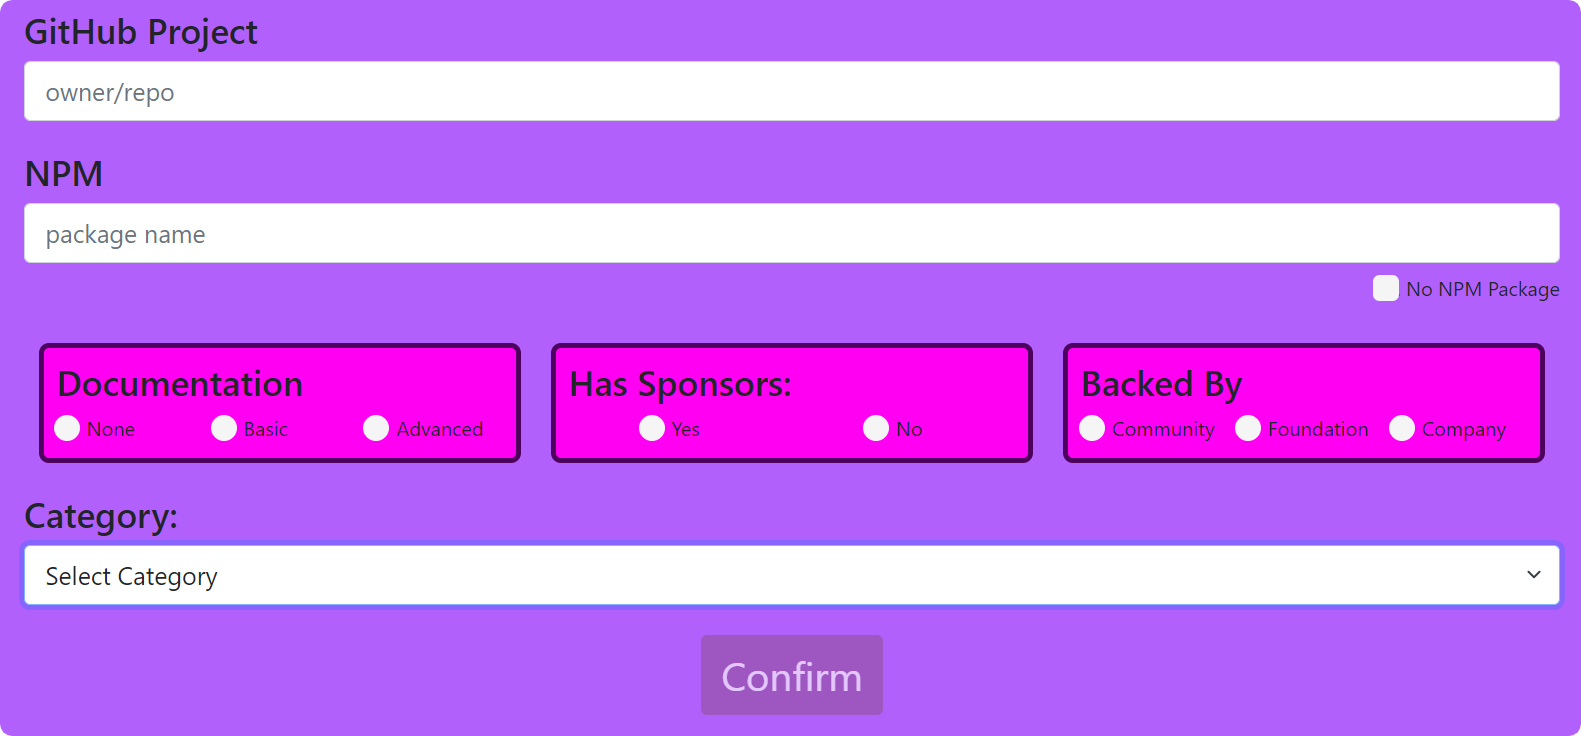
\includegraphics[scale=0.25]{figures/04/WebInterface.png}
    \caption{Web-Interface}
    \label{abb:Web_Interface}
\end{figure}



% ----------------------------------------- Dokumentation ---------------------------------------- %
\subsection{Dokumentation} \label{ssec:manuelle_datenerfassung_dokumentation}
Die Dokumentation des Projektes wurde analysiert und nachfolgenden Kriterien kategorisiert:

\begin{itemize}[noitemsep]
    \item[0 =] keine Dokumentation
    \item[1 =] basis Dokumentation, rein textuell
    \item[2 =] Dokumentationen mit Demos oder Live-Beispielen,
        Einführungsvideos oder ähnliches
\end{itemize}


% ------------------------------------------- Sponsoren ------------------------------------------ %
\subsection{Sponsoren}
Für jedes Projekt wurde geprüft, ob es Sponsoren hat. Die Anzahl an Sponsoren bzw. die Einnahmen
durch Sponsoren wurden nicht beachtet. Das Vorhandensein der Sponsoren wurde wie folgt codiert:

\begin{itemize}[noitemsep]
    \item[0 =] hat keine Sponsoren
    \item[1 =] hat Sponsoren
\end{itemize}


% ------------------------------------------- Backed by ------------------------------------------ %
\subsection{Kategorisierung der Mitwirkenden} % TODO KAPITEL UMBENNENEN


Im nächsten Schritt wurde vermerkt wer hinter einem Projekt steht, hierbei wurde in drei Kategorien
eingeteilt:

\begin{itemize}[noitemsep]
    \item[0 =] Eines reines Community Projekte, welches unabhängig von Unternehmen ist. Beispiel: VueJS.
    \item[1 =] Von einer Stiftung wie OpenJS\footnote{\url{https://openjsf.org/}} unterstütztes oder
        entwickeltes Projekt.\\ Beispiel: NodeJS.
    \item[2 =] Projekte die von Unternehmen entwickelt werden, wie React von Facebook beispielsweise.
\end{itemize}

\noindent
Diese Information fanden sich entweder auf der GitHub-Page, Homepage des Projektes oder das Unternehmen
ist der Besitzer des Repositories.



% ------------------------------------------- Kategorie ------------------------------------------ %
\newpage %! NewPage
\subsection{Projektarten}
Im letzten Schritt wurde das Projekt in eins der folgenden Kategorien zugeordnet:

\begin{multicols}{2}
    \begin{itemize}
        \setlength\itemsep{0em}
        \item Utility
        \item UI
        \item Application
        \item Library
        \item Framework
        \item Test-Framework
        \item Open-Core
        \item API
    \end{itemize}
\end{multicols}

% Erläuterung der Kategorien
\subsubsection*{Erläuterung der Kategorien}

\begin{itemize}
    \setlength\itemsep{0em}
    \item \textbf{Utility}, wurden Projekte kategorisiert, die nicht direkt in Projekte eingebaut
          werden, sondern als Tool verwendet werden. Beispiel: \texttt{shelljs/shelljs}\footnote{
              \url{https://github.com/shelljs/shelljs}}
    \item \textbf{Application}, sind eigenständige Produkte wie draw.io\footnote{
              \url{https://github.com/jgraph/drawio}}
\end{itemize}





% ------------------------------------------------------------------------------------------------ %
%                                                                                                  %
%                                   Automatisierte Datenerfassung                                  %
%                                                                                                  %
% ------------------------------------------------------------------------------------------------ %
\newpage %! newpage
\section{Automatisierte Datenerfassung}\label{sec:automatisierte_datenerfassung}

Im zweiten Teil der Erhebung wurden weitere Daten automatisiert gesammelt. Hierfür wurde die
GitHub API\footnote{\url{https://docs.github.com/en/rest}}, NPM
API\footnote{\url{https://github.com/npm/registry}} und für einige Daten Web-Scraping
verwendet.

Zu diesem Zweck wurde eine weitere NodeJS Applikation geschrieben, welche die CSV-Datei aus dem
Kapitel \ref{sec:manuelle_datenerfassung} ausliest und mithilfe der APIs und Web-Scraping eine neue
CSV-Datei generiert. In Abbildung \ref{abb:Architektur} wird der Prozess der Datenerhebung grafisch
dargestellt. In den folgenden Unterkapiteln wird aufgelistet welche Daten mittels welcher Methode gesammelt wurden.


% ----------------------------------- Daten aus der GitHub API ----------------------------------- %
\subsection{Daten aus der GitHub API}
Mittels der GitHub API wurden folgende Daten gesammelt:

\begin{itemize}[noitemsep]
    \item Anzahl der GitHub-Sternen
    \item Erstellungsdatum des Repositories
    \item Vorhandensein einer \textit{CODE\_OF\_CONDUCT.md}
    \item Vorhandensein einer \textit{CONTRIBUTING.md}
    \item Lizenz
    \item Anzahl der Commits in den letzten 12 Monaten
    \item Anzahl der Issues in den letzten 12 Monaten
\end{itemize}

% * GitHub_generalInfo
% * projectHealth
% * commitActivity
% * issues_PRs

% ------------------------------------- Daten aus der NPM API ------------------------------------ %
\subsection{Daten aus der NPM API}
Mit der NPM API wurden die Downloads der letzten 7 Tage abgefragt.

% * npm_downloads

% ---------------------------------- Daten aus dem Web-Scraping ---------------------------------- %
\subsection{Daten aus dem Web-Scraping}
Mithilfe von Web-Scraping wurden folgende Daten erfasst:

\begin{itemize}[noitemsep]
    \item Die Anzahl von \textit{UsedBy} auf der GitHub Page des Projektes.
    \item Anzahl der Gesamt-Commits auf dem default Branch
    \item Anzahl der Mitwirkenden
\end{itemize}

\subsubsection*{Anmerkung:}
Ein Mitwirkender zählt nur dann als solcher, wenn dessen Commit entweder auf dem \textit{default}
oder \textit{gh-pages} Branch liegt. Die Commits auf anderen Branches werden nur dann gezählt,
wenn ein merge auf einen der vorherig erwähnten Branches stattfindet. Gleiches gilt für Commits \cite{GHapiDocsCommits}.

% * GitHub_usedBy
% * GitHub_Page
% * npm_dependants


% ----------------------------------- Nachbearbeitung der Daten ---------------------------------- %
\subsection{Nachbearbeitung der Daten}

Nachdem erheben der Daten war eine Nachbearbeitung notwendig. Einige Projekte hatten die Lizenz
\texttt{other}. Der Grund hierfür ist, dass die \texttt{LICENSE.md} nicht dem Standardtext einer
Lizenz entsprochen hat. Ein Beispiel wäre die Lizenz von
meteor\footnote{\url{https://github.com/meteor/meteor/blob/devel/LICENSE}},
welche nach dem offiziellen Lizenztext noch eine Anmerkung bezüglich benutzter Bibliotheken hat.
Alle als \texttt{other} gekennzeichneten Projekte wurden manuell geprüft und korrigiert.
%
Zudem wurden Projekte ohne Lizenzen oder Lizenzen die nicht von der \textit{Open Source Initiative}
zugelassene sind komplett aussortiert.
%
Nach dem gleichen Prinzip wurden Projekte kontrolliert, die laut API kein Contributing Guide bzw. kein Code
of Conduct haben. Grund hierfür ist, dass GitHub das Vorhandensein dieser Dateien nur dann erkennt,
wenn diese im Hauptverzeichnis liegen und exakt \texttt{CONTRIBUTING.md} bzw \texttt{CODE\_OF\_CONDUCT.md}
heißen. Einige Projekte hatten Tippfehler in den Dateinamen oder den Contributing Guide bzw Code of Conduct
war Teil der README.md statt eine eigene Datei bzw. auf der Website des Projektes.
% 9 Datensätze wurden korrigiert (Contributing) / 2 Datensätze wurden bezüglich (CoC) korrigiert





% ------------------------------------ Abbildung: Architektur ------------------------------------ %
\begin{figure}[h]
    \centering
    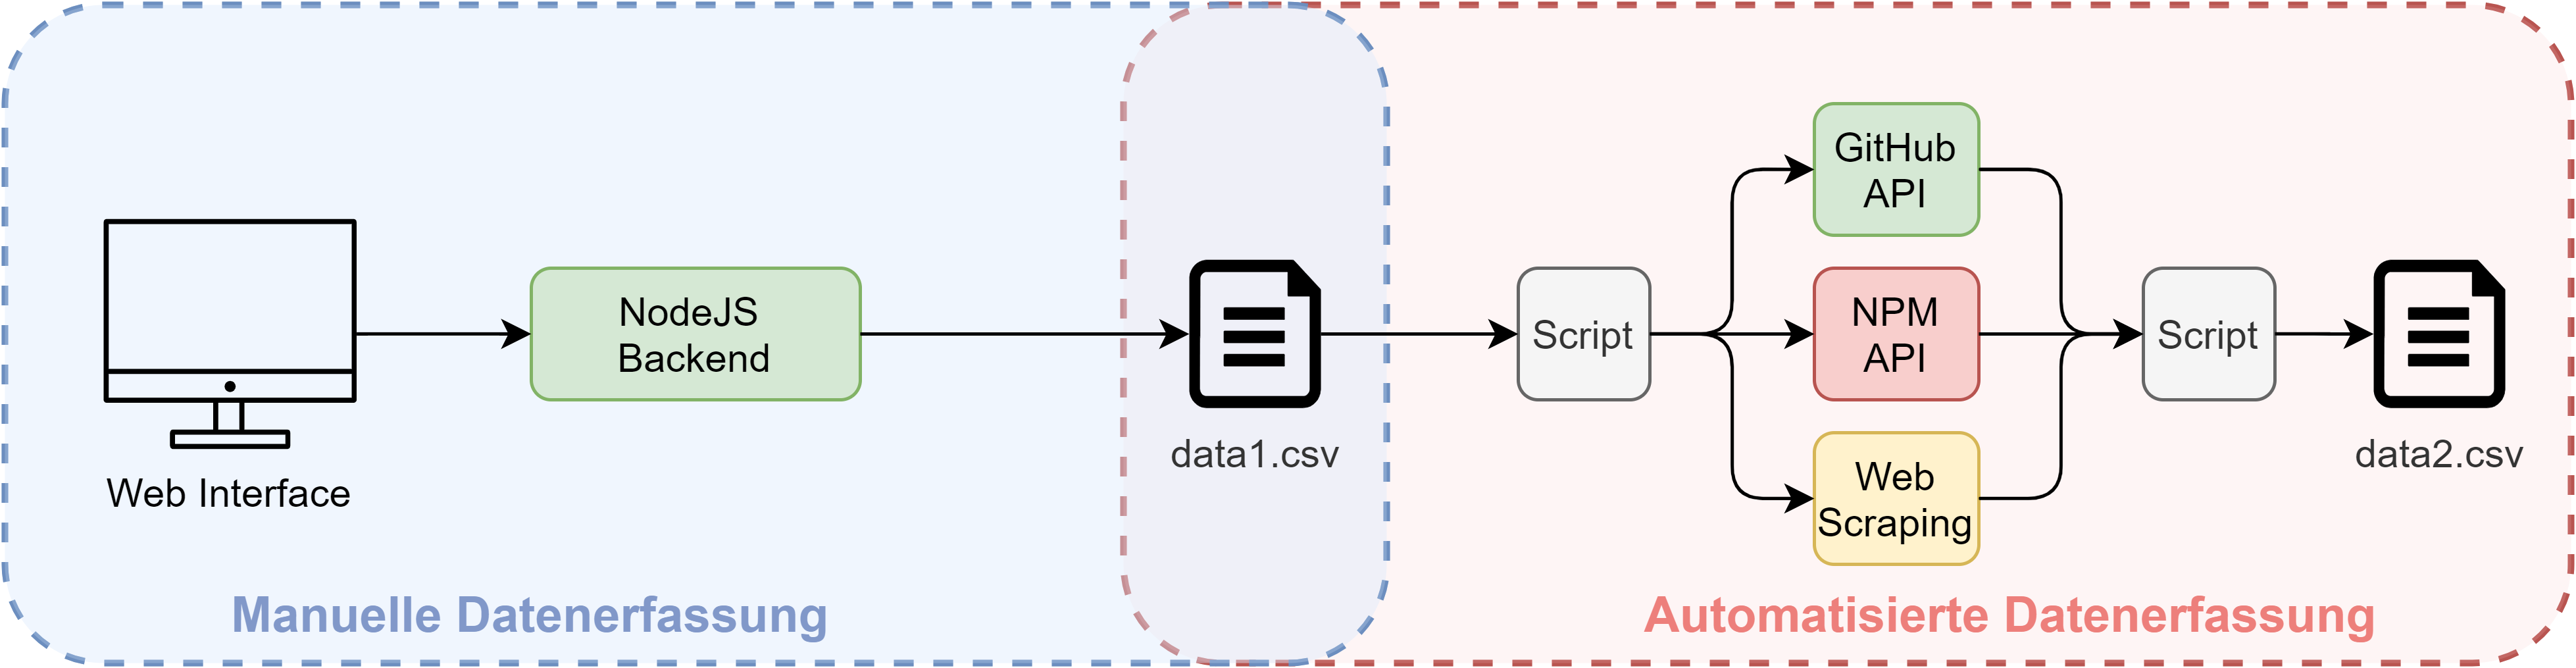
\includegraphics[scale=0.1]{figures/04/DatenerfassungArchitektur.png}
    \caption{Prozess der Datenerhebung}
    \label{abb:Architektur}
\end{figure}


% \section{Top 100 Projekte}\label{sec:top_100_projects}

% \xodoo{Datenerhebubg der Top 100 Projekte, unabhängig von Programmiersprache. Ziel: Besseren eindruck
% über Lizenzen. Vorgehen: Wie zuvor auch, keine Tutorials etc. Abgespeckte Version weil die meisten
% "Funktionen" des Haversters abgeschaltet wurdens sind.}

% Hier wird die Regel "Nur JS" gebrochen, da das Ziel ist GH-Sterne in Relation zu den Lizenzen zu 
% vergleichen.
\newpage %! newpage
\chapter{Analyse der erhobenen Daten}


% ------------------------------------------- Lizenzen ------------------------------------------- %
\section{Lizenzen}

\todo{Verweis auf Kapitel 2.1 Lizenzen => Warum genau diese Aufteilung}

\todo{Bonus Formulierung: Die Projekte die offen sind befinden sich in den Top 50\%....}

\bigskip
\noindent
Zunächst wurden die Datensätze in zwei Gruppen aufgeteilt, Projekte mit freizügigen und restriktiven
Lizenzen. \todoo{Die Aufteilung erfolgt hierbei wie im Kapitel 1.3.3.7 zu Lizenzen näher erklärt wurde.}
In der Tabelle \ref{tab:lizenzen} findet sich eine Zusammenfassung aller Lizenzen der
Projekte die erfasst worden sind. Wie man erkennt haben 91\% der Projekte eine freizügige Lizenz, wobei
die MIT Lizenz mit 69\% die beliebteste aller Lizenzen ist. Um die Beliebtheit der Projekte zu
vergleichen wurden die GitHub Sterne als Metrik verwendet.
Aufgrund der stark ungleich großen Gruppen wurden anhand von Gruppen anhand von Ranking verglichen.
Hierfür wurden die Projekte, wie in Abbildung \ref{abb:permissive_vs_restriktiv_BarChart} zu sehen
ist, absteigend nach Anzahl der Sterne sortiert.
Das erste Projekt mit einer restriktive Lizenz belegt hierbei den Platz 35. Projekte mit freizügige
Lizenzen übertreffen die restriktiven sowohl in der Menge als auch in ihrer Beliebtheit.
%
%
%
% Daten von GitHub
% In 2015 hat GitHub in einem Blogeintrag die Aufteilung der Lizenznutzung auf ihrer Platform veröffentlicht
% \cite{OpenSourceLicense2015}. Wie man in Tabelle \ref{tab:GitHub_Blog_Lizenznutzung2015} sehen kann,
% haben 64\% aller Projekte permissive Lizenzen und 24\% restriktive. 15\% der Projekte haben keine
% Standardlizenz und werden von GitHub daher als \textit{other} kategorisiert.
%
%
% \subsubsection*{Anmerkung:}
% Die Tabelle \ref{tab:GitHub_Blog_Lizenznutzung2015} ergibt in der Summe über 100\%. Grund hierfür
% könnte sein, dass einige Projekte Dual Lizenzen besitzen
%
% H1 Bestätigt sich.
Somit bestätigt sich die \hyperref[H:1]{Hypothese H1}. Projekte mit freizügigen Lizenzen sind
beliebter als Projekte mit restriktiven Lizenzen.


% \bigskip
% \noindent
% % Top 100 Projekte
% Um auszuschließen das es sich hierbei, um ein Phänomen handelt welches sich nur bei den
% Programmiersprachen JS/TS wiederfindet wurden, wie in \ref{sec:top_100_projects} beschrieben,
% die Top 100 GitHub Projekte separat erfasst. Wie sich in Tabelle \ref{tab:top_100}
% zeigt ist die MIT Lizenz mit 58\% die am häufigsten verwendete Lizenz gefolgt von Apache 2.0 (24\%)
% und der BSD-3-Clause (8\%).
% Insgesamt sind 93\% der Top 100 Projekte auf GitHub permissiv lizenziert.


% NPM Downloads
Ursprünglich sollten auch die NPM Downloads als Beliebtheitsmerkmalen verwendet und vergleichen
werden. Allerdings handelt es sich bei restriktiven Projekten meist um Applikationen, dies hat zur
Folge, dass diese Projekte nicht auf npm gelistet sind.  % 4 von 10 sind Applikationen



% ------------------------------------------ Hypothese 2 ----------------------------------------- %
\bigskip
\noindent
Um die zweite Hypothese zu prüfen wurden ähnlich vorgegangen, für diesen Vergleich wurden Anzahl der
Contributor sowie Commits betrachtet. Vergleicht man die Anzahl der Contributor liegt das erste
restriktive Projekt auf Platz 51. Ganz anders sieht es aus, wenn man die Commits vergleicht.
Wie man in Abbildung \ref{abb:license_vs_commits} sehen kann befinden sich zwei Projekte mit
restriktiven Lizenzen unter den Top 20, auf Platz 9 und 19.

Die Vermutung das freizügige Lizenzen zu mehr technischem Erfolg führen wird daher nur zum Teil
unterstützt. \todoo{Freizügige Lizenzen ziehen zwar tendenziell mehr Mitwirkende, allerding leisten
    die Contributor von restriktiven Projekten vergleichsweise viel Arbeit.}



% Lizenzen der erfassten Projekte
\begin{table}[h]
    \begin{tabular}{lcllc}
        \cline{1-2} \cline{4-5}
        \textbf{Permissive Lizenz} & \multicolumn{1}{l}{Anz.} & \hspace{2cm} & \textbf{Restriktive Lizenz} & \multicolumn{1}{l}{Anz.} \\ \cline{1-2} \cline{4-5}
        MIT                        & 74                       &              & AGPLv3                      & 4                        \\
        Apache 2.0                 & 18                       &              & GPLv3                       & 3                        \\
        BSD 3-Clause               & 3                        &              & LGPLv2.1                    & 1                        \\
        BSD 2-Clause               & 2                        &              & OSLv3.0                     & 1                        \\
        ISC                        & 1                        &              & LGPLv3                      & 1                        \\ \cline{1-2} \cline{4-5}
        \textit{Gesamt}            & 98                       &              & \textit{Gesamt}             & 10
    \end{tabular}%
    \caption{Lizenzen der erfassten Projekte}
    \label{tab:lizenzen}
\end{table}

% Tabelle aus vom GitHub Blogpost & Top 100
\begin{table}[]
    \begin{tabular}{clc}
        \hline
        \multicolumn{1}{l}{Rang} & Lizenz      & \multicolumn{1}{l}{\% der Projekte} \\ \hline
        1                        & MIT          & 44,69\%                            \\
        2                        & Other        & 15,68\%                            \\
        3                        & GPLv2        & 12,96\%                            \\
        4                        & Apache       & 11,19\%                            \\
        5                        & GPLv3        & 8,88\%                             \\
        6                        & BSD 3-Clause & 4,53\%                             \\
        7                        & Unlicense    & 1,87\%                             \\
        8                        & BSD 2-clause & 1,70\%                             \\
        9                        & LGPLv3       & 1,30\%                             \\
        10                       & AGPLv3       & 1,05\%
    \end{tabular}%
    \caption{GitHub Blogeintrag: Lizenznutzung 2015}
    \label{tab:GitHub_Blog_Lizenznutzung2015}
\end{table}

\begin{table}[]
    \begin{tabular}{clc}
        \hline
        \multicolumn{1}{l}{Rang} & Lizenz       & \multicolumn{1}{l}{Anzahl der Projekte} \\ \hline
        1                        & MIT          & 58                                      \\
        2                        & Apache       & 24                                      \\
        3                        & BSD 3-Clause & 8                                       \\
        4                        & GPLv3        & 4                                       \\
        5                        & GPLv2        & 2                                       \\
        6                        & BSD 2-Clause & 1                                       \\
        7                        & ISC          & 1                                       \\
        8                        & MLP 2.0      & 1                                       \\
        9                        & AGPLv3       & 1
    \end{tabular}%
    \caption{Lizenzen der Top 100 GitHub Projekte}
    \label{tab:top_100}
\end{table}


% Abbildung: Lizenzen vs Lizenzen
\begin{figure}[]
    \centering
    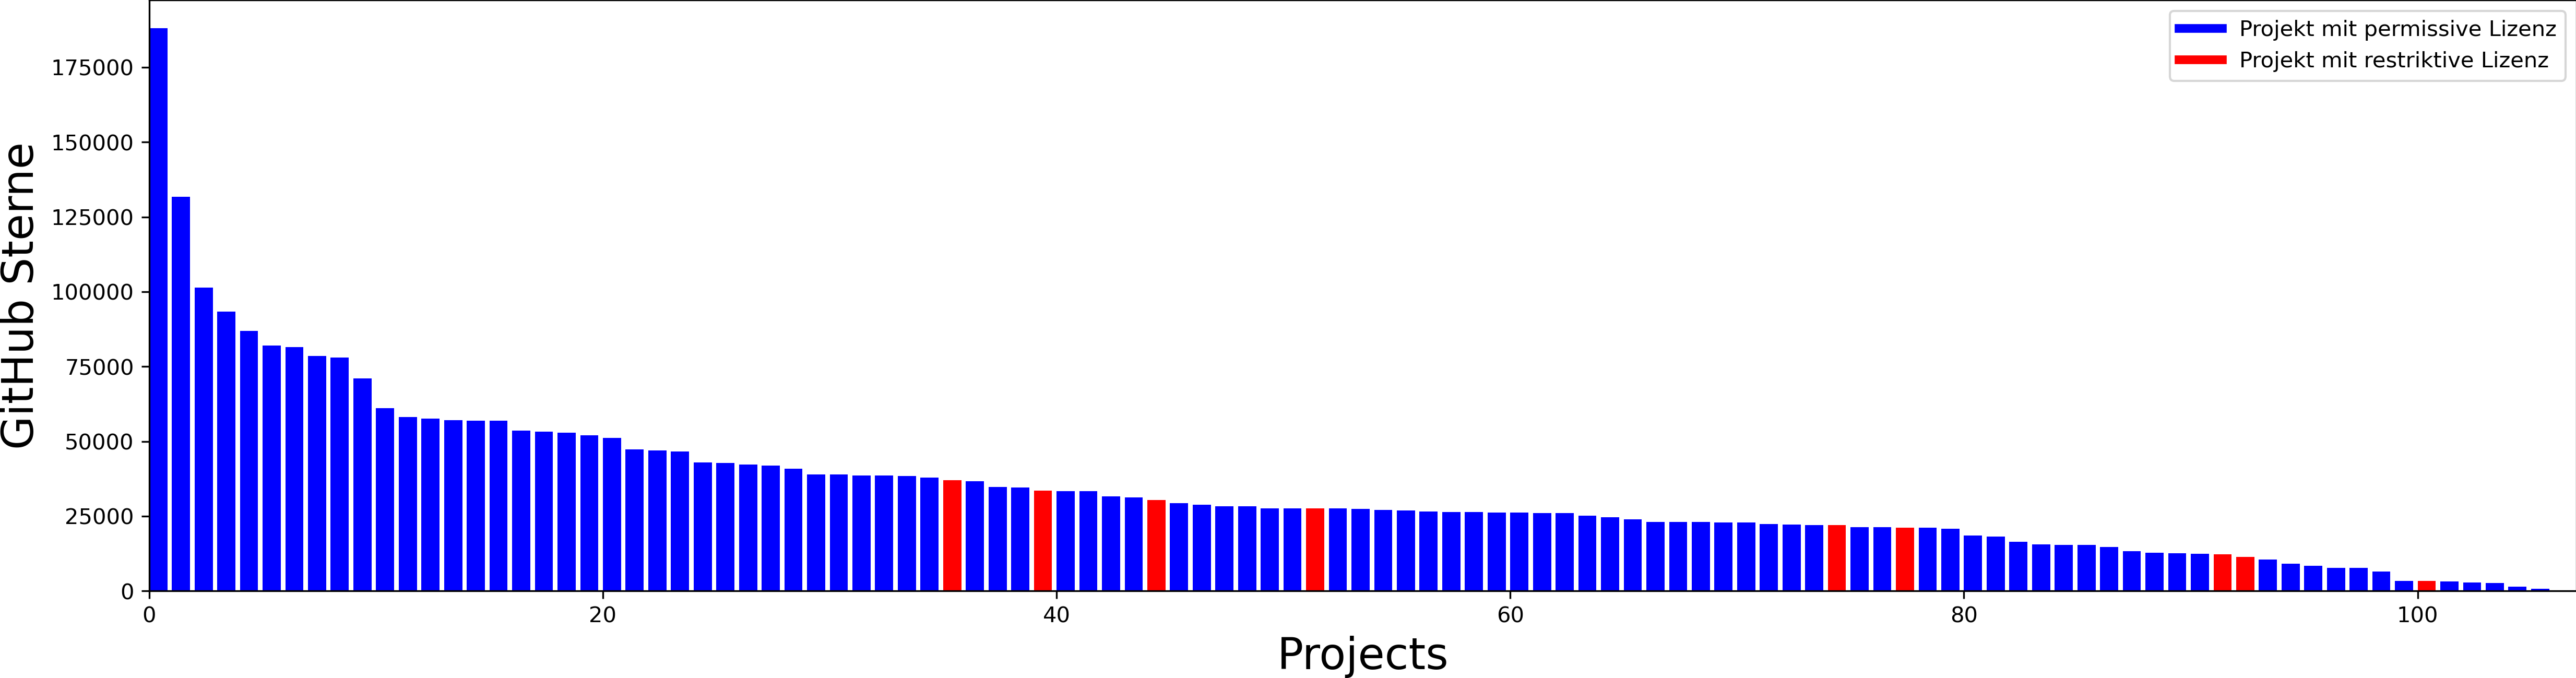
\includegraphics[scale=0.4]{figures/05/permissive_vs_restrictive_asBarChart.png}
    \caption{Effekt von Lizenzen auf GitHub Sterne}
    \label{abb:permissive_vs_restriktiv_BarChart}
\end{figure}

% Abbildung: Lizenzen vs Commits
\begin{figure}[]
    \centering
    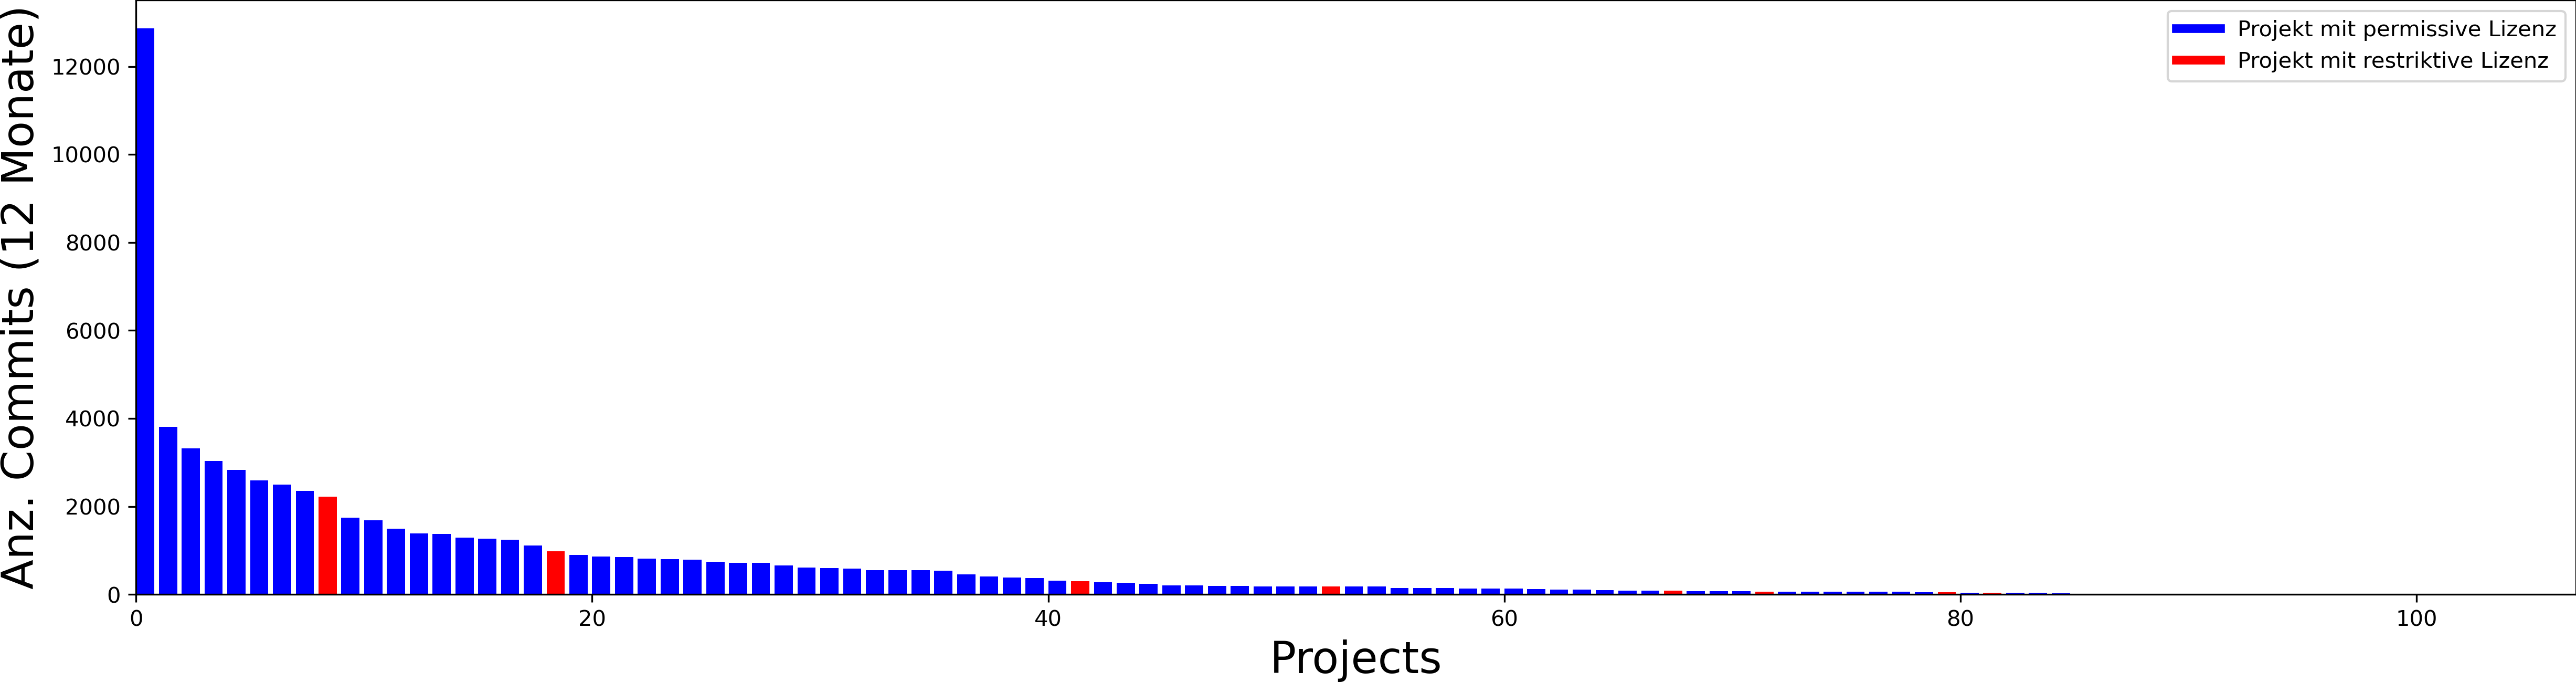
\includegraphics[scale=0.4]{figures/05/license_vs_last12MonthsCommits_asBarChart.png}
    \caption{Effekt von Lizenzen auf Anzahl der Commits}
    \label{abb:license_vs_commits}
\end{figure}



% ---------------------------------------- Code of Conduct --------------------------------------- %
\newpage %! newpage
\section{Code of Conduct}\label{sec:CoC}
Der Datensatz wurde hier erneut in zwei Gruppen geteilt, Projekte mit Code of Conduct und Projekte
ohne. Verglichen wurden GitHub Sterne und Downloadzahlen mittels Median. Der Median wurde in diesem
Fall gewählt, da sowohl Sterne als auch Downloads starke Ausreißer haben. Da nicht alle Projekte auf
NPM gelistet sind, beispielsweise Applikationen, wurden diese bei der Berechnung des Medians der
Downloadzahlen nicht berücksichtigt. So bildet sich der Median der Sterne aus 108  Datensätzen
und der Median der Downloads aus 88 Datensätzen.

Wie man in Tabelle \ref{tab:relation_CoC_Popularity} zu erkennen ist haben 53\% der Projekte einen
Code of Conduct.
Projekte mit Code of Conduct haben 51\% mehr Downloads auf NPM und 55\% mehr Github Sterne.
Da Projekte mit einem Code of Conduct beliebter sind, als die ohne bestätigt sich somit
\hyperref[H:4]{Hypothese H4}


\begin{table}[h]
    \begin{tabular}{l|c|c|}
        \cline{2-3}
                                  & \multicolumn{1}{l|}{\textbf{Projekte mit Code of Conduct}} & \multicolumn{1}{l|}{\textbf{Projekte ohne Code of Conduct}} \\ \hline
        \textbf{Anzahl}           & 57                                                         & 51                                                          \\ \hline
        \textbf{Median Sterne}    & 34.581                                                     & 22.279                                                      \\ \hline
        \textbf{Median Downloads} & 1.636.148,5                                                & 1.078.509,5                                                 \\ \cline{2-3}
    \end{tabular}%
    \caption{Relation von Code of Conduct und Beliebtheit}
    \label{tab:relation_CoC_Popularity}
\end{table}


% \begin{figure}[h]
%     \centering
%     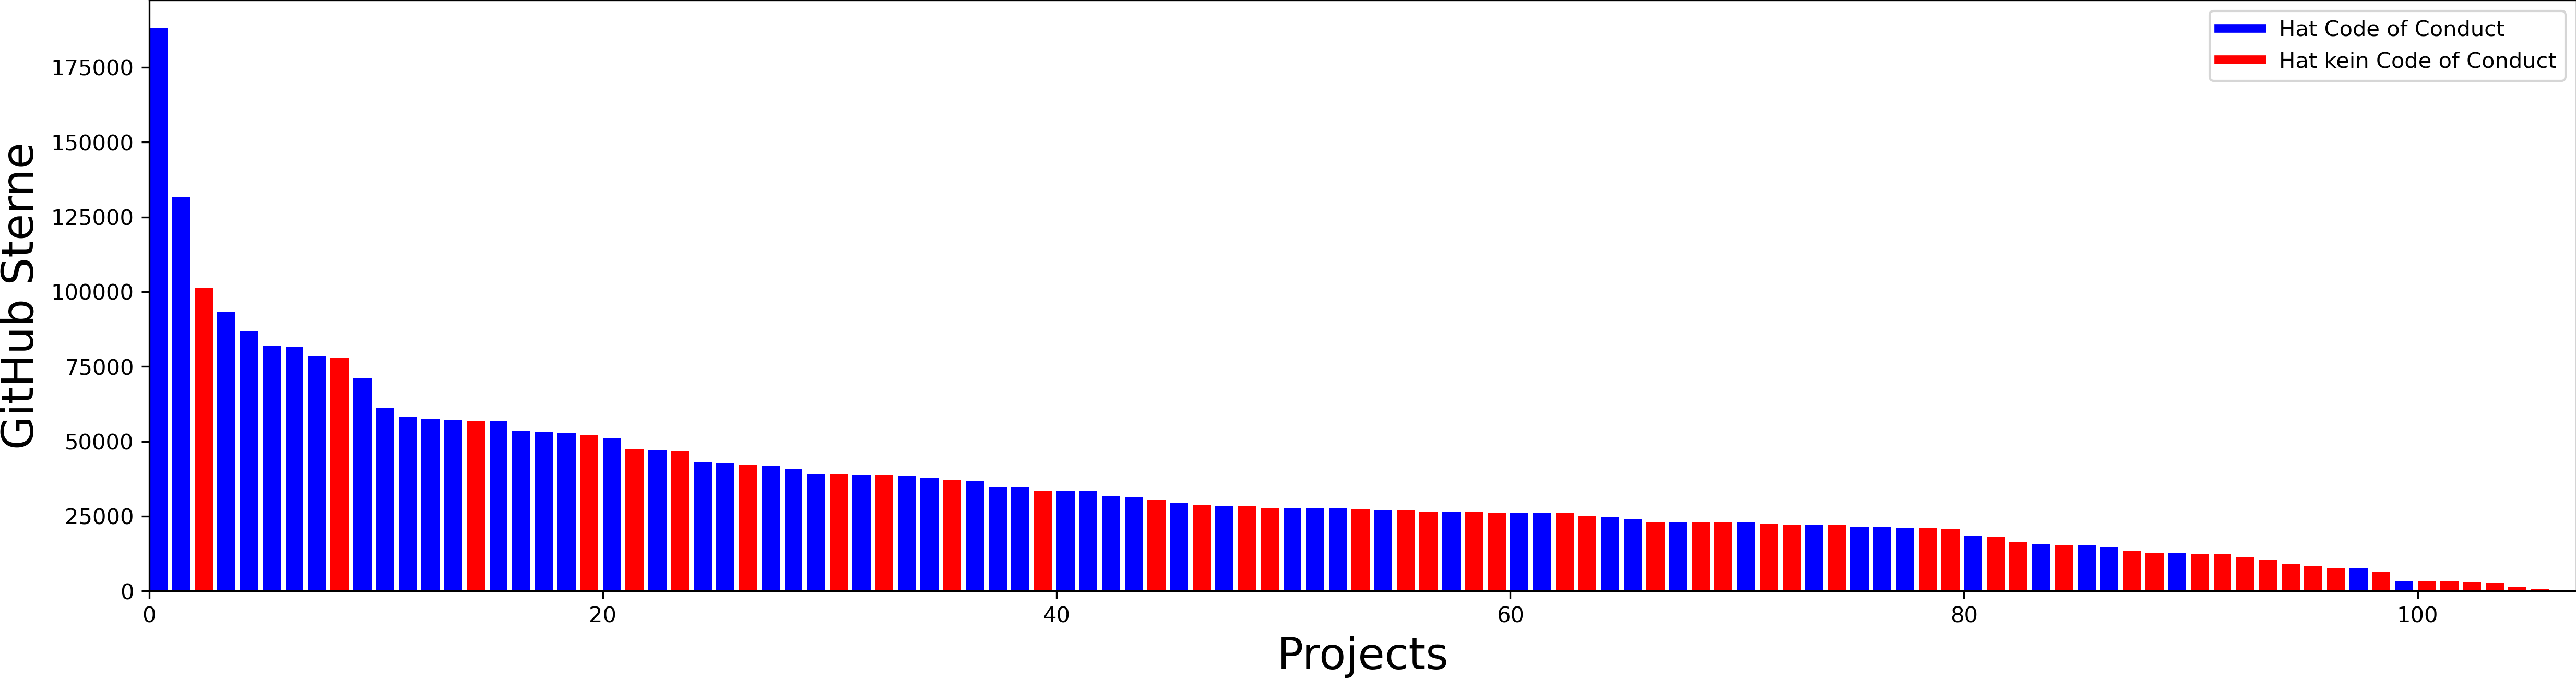
\includegraphics[scale=0.42]{figures/05/Stars_vs_CoC_asBarChart.png}
%     \caption{Einfluss von Code of Conduct auf Sterne}
%     \label{abb:CodeOfConduct_Stars}
% \end{figure}



% -------------------------------------- Contributing Guide -------------------------------------- %
\section{Contributing Guide}

\todo{Bonus Formulierung: Die Projekte die ein CG haben befinden sich in den Top 50\%....}

Wie im Kapitel \ref{sec:CoC} wurde auch hier der Datensatz in zwei Gruppen unterteilt. Projekte mit
und ohne einen Contributing Guide (CG). Hier soll der Zusammenhang zwischen dem Vorhandensein eines
CG und Anzahl der Contributor bzw. Commits \todoo{erforscht} werden.

Hierbei beschränken sich die Anzahl der Commits auf die letzten 12 Monate, um eine vergleichbare
Basis zu schaffen. Gleiches war bei den Contributor nicht umsetzbar, da die GitHub API keinen
Endpoint hierfür hat, somit werden Contributor über den gesamten Zeitraum des Projektes verglichen.

Anders als beim Code of Conduct, haben hier 86\% aller Projekte einen (CG).
In Abbildung \ref{abb:ContributingGuide_vs_Contributors} werden die Projekte nach Anzahl der Contributor
sortiert, wie man erkennen kann haben die Projekte mit den meisten Mitwirkenden alle einen CG. Das
erste Projekt ohne belegt hier Platz 54. Nach dem gleichen Schema wurden auch nach Anzahl der Commits
sortiert, das erste Projekt ohne CG landet hier auf Platz 42.

In beiden vergleichen platzieren sich Projekte mit CG weit vor Projekten ohne. Wie in \hyperref[H:5]
{Hypothese H5} angenommen hat der Contributing Guide einen positiven Effekt auf den technischen Erfolg.

\begin{figure}[h]
    \centering
    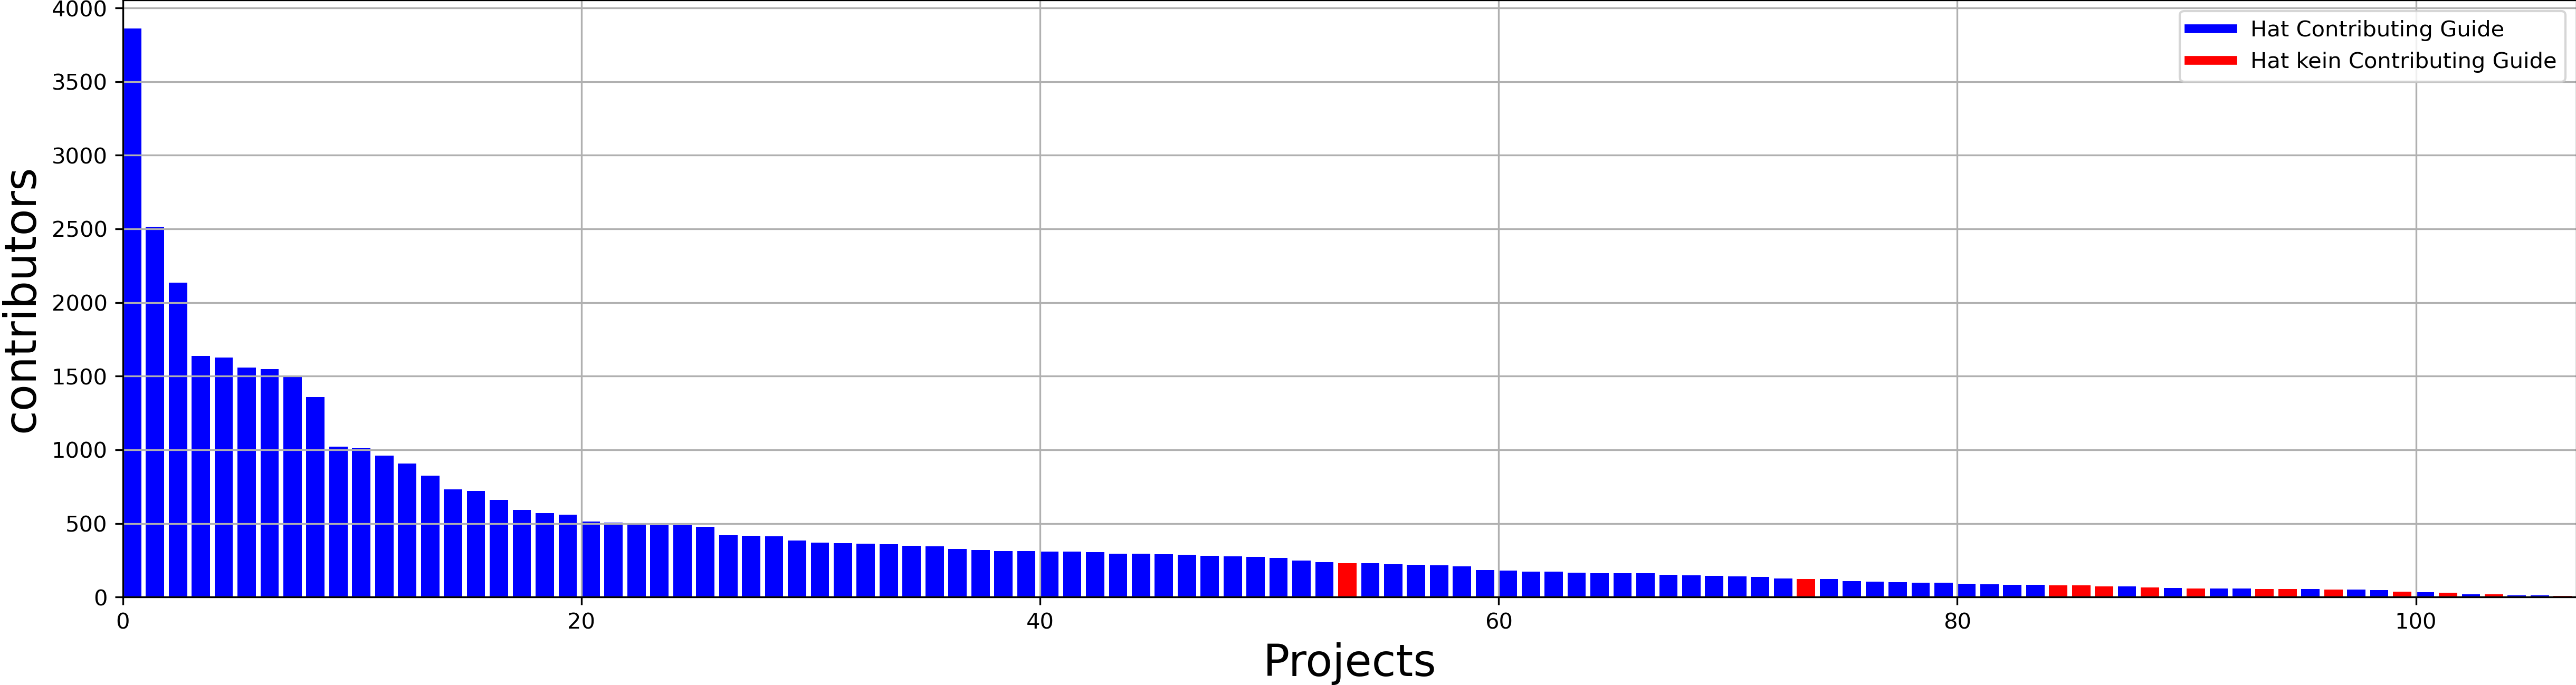
\includegraphics[scale=0.42]{figures/05/Contributors_Projects_asBarChart.png}
    \caption{Einfluss von Contributing Guide auf Contributor}
    \label{abb:ContributingGuide_vs_Contributors}
\end{figure}

\newpage %! new Page
\section{Einfluss von Sponsoren auf den technischen Erfolg}

Erneut wurde der Datensatz in zwei Gruppen geteilt, Projekte mit und ohne Sponsoren. Verglichen wurde
der Median der Commits der letzten 12 Monate sowie die Anzahl an Contributor. In Tabelle \ref{}

\begin{table}[h]
    \begin{tabular}{l|c|c|}
        \cline{2-3}
                                                      & \multicolumn{1}{l|}{\textbf{Projekte mit Sponsoren}} & \multicolumn{1}{l|}{\textbf{Projekte ohne Sponsoren}} \\ \hline
        \textbf{Anzahl der Projekte}                  & 56                                                   & 52                                                    \\ \hline
        \textbf{Median Anz. Sterne}                   & 26.468                                               & 27.551                                                \\ \hline
        \textbf{Median Anz. Downloads}                & 1.409.792                                            & 1.094.063                                             \\ \hline
        \textbf{Median Commits der letzten 12 Monate} & 221                                                  & 128                                                   \\ \hline
        \textbf{Median Anz. Contributor}              & 289                                                  & 155                                                   \\ \hline
    \end{tabular}%
    \caption{Relation von Sponsoren und Erfolg}
    \label{tab:Sponsors_vs_NonSponsors}
\end{table}

- Bisschen Tricky weil manche keinen Sponsor haben aber dafür von Unternehmen her aus kommen.\\
- Hier könnte man die Hypothese ändern auf "Finaziell unterstützte Projekte sind erfolgreicher"
dann schließt man nämlich auch die Unternehmen und Foundations mit ein und dann easy. Dann fasst man einfach
Sponsor == 1 mit, BackedBy == 1, BackedBy == 2 zusammen und gute Nacht. Hier wird es evtl möglich sein
wieder mit Median etc zu arbeiten, je nachdem wie spread die daten sind.
\chapter{Umfrage}


% Introduction Umfrage
Als Ergänzung zur Datenerfassung der GitHub Projekte wurde auch eine Umfrage durchgeführt.
Ziel der Umfrage war es herauszufinden worauf die Nutzer von Open Source achten, wenn sie ein Projekt
wählen. Das übergeordnete Ziel war es die Hypothesen H3, \todoo{(H6)}, H7 und H9 zu prüfen.
An der Online-Umfrage haben Softwareentwickler der adesso SE, sowie Studenten der TH Rosenheim teilgenommen.
Insgesamt erhielt die Umfrage 308 Antworten. Zur Erstellung der Umfrage wurde \textit{cryptpad.org} 
verwendet \cite{Cryptpad_org}.

Hierbei sollten die Teilnehmer Aussagen zu den Thema Dokumentation, Beliebtheit, Sponsoren und
Entwicklung bewerten. Als Bewertungsskala wurde eine 5-Punkte Likert-Skala verwendet \cite{likertScale}.

\todoo{Interpretation der Durchschnitte: 1 = der Teilnehmende stimmt der Aussage gar nicht zu, 5 =
    der Teilnehmende stimmt der Aussage vollkommend zu. 3 = Undecided, doesnt matter etc.}



% Dokumentation
\newpage
\section{Dokumentation}

% Was mussten die Teilnehmer machen?
Im ersten Teil der Umfrage mussten die Teilnehmenden zu zwei Aussagen verschiedene Kriterien bewerten.
Diese Kriterien wurden gewählt basierend auf Erfahrung als Entwickler als auch Beobachtungen vieler
Dokumentationen während der manuellen Datenerfassung zu aus Kapitel
\ref{ssec:manuelle_datenerfassung_dokumentation}.


\bigskip
\noindent
Die erste Aussage war \textit{"Wie wichtig sind Ihnen folgende Aspekte der OSS-Dokumentation"}, mit den Punkten:
\begin{multicols}{2}
    \begin{itemize}
        \setlength\itemsep{0em}
        \item Übersichtlichkeit
        \item Einfache Sprache
        \item Live-Demos
        \item Übersetzungen (z.B. Englisch -> Deutsch)
        \item Das Vorhandsein einer Getting Started Page
        \item Code Beispiele
        \item Strukturierung der Dokumentation
        \item []
    \end{itemize}
\end{multicols}

\bigskip
\noindent
Die zweite Aussage war \textit{"Die folgenden Punkte würden mich von der Nutzung eines OSS-Projekts
    abhalten oder mich möglicherweise dazu veranlassen, nach Alternativen zu suchen."}, mit den Punkten:

\begin{multicols}{2}
    \begin{itemize}
        \setlength\itemsep{0em}
        \item Keine Code Beispiele
        \item Schlecht strukturierte Dokumentation
        \item Dokumentation zu komplex
        \item Fehlende Übersetzung (z.B. fehlende deutsche Übersetzung)
        \item Fehlende Getting Started Page
    \end{itemize}
\end{multicols}



\bigskip
\noindent
% More Detail
Die Aussagen wurden auf einer 5-Punkte Skala bewertet, hierbei entspricht 1 \textit{Stimme gar nicht zu}
und 5 \textit{Stimme vollkommen zu}. Um die Aussagen miteinander zu vergleichen, wurde jeweils der
Mittelwert berechnet.

% Conclusion
Die zwei wichtigsten Aspekte einer Guten Dokumentation sind laut den Befragten, Code Beispiele und
Übersichtlichkeit in beiden Fällen mit einem durchschnittlichen Wert von 4,36. Gefolgt von guter 
Struktur (4,09) und
das Vorhandensein eines \textit{Getting Started} (3,98). Einfache Sprache (3,08) und Live-Demos spielt für
die Befragten eine weniger wichtige Rolle. 
Übersetzungen belegen mit 1,53 den letzten Platz und spielt somit die unwichtigste Rolle in einer 
guten Dokumentation. 


Die zweite Aussage war \textit{"Die folgenden Punkte würden mich von der Nutzung eines OSS-Projekts
    abhalten oder mich möglicherweise dazu veranlassen, nach Alternativen zu suchen."} Am höchsten bewertet
wurde der Punkt \textit{Fehlende Code Beispiele} (4,07) und ist somit der wichtigste Teil einer guten
Dokumentation, gefolgt von schlechter Struktur (3,91). 
Eine komplexe Dokumentation oder das Fehlen einer Getting Started Seite wurde hierbei als mittelmäßig kritisch 
eingestuft, mit einer durchschnittlichen Bewertung von 3,29 bzw. 3,10. Das Fehlen einer Übersetzung ist mit 1,37
das unwichtigste Kriterium.
In den Abbildungen \ref{abb:GuteDoku_BarChart} und
\ref{abb:SchlechteDoku_BarChart} wird das Meinungsbild der Teilnehmer grafisch dargestellt.

% Interpretation beider Fragen.
Zusammenfassend kann man sagen, dass Code Beispiele ein Must Have einer Dokumentation ist.
Das Vorhandensein wird als wichtig eingestuft, während das Fehlen dazu führen könnte, dass Nutzer
zu alternativen greifen würden. Übersetzungen hingegen werden als gleichgültig betrachtet, das
Vorhandensein bietet wenig Mehrwert, die Abwesenheit wird nicht als kritisch betrachtet.

% ---------------------------------------------------- %
% Likert to Kano (kinda)
% https://www.eric-klopp.de/texte/die-kano-methode.php
% ---------------------------------------------------- %


% ----------------------------------------- FreitextFeld ----------------------------------------- %
\bigskip
\noindent
Beide Fragen hatten jeweils ein Freitextfeld, indem die Teilnehmenden die Möglichkeit hatten weitere
Aspekte einer guten bzw. schlechten Dokumentation zu nennen. Diese Freitextfelder waren optional und
wurden von 95 bzw. 71 der gesamten 308 Teilnehmenden genutzt.
Alle Einträge wurden kategorisiert und zusammengefasst.

% Most Used Words
In der Tabelle \ref{tab:freitext_felder_ergebnisse} finden sich die am häufigsten genannten
Punkte. Aktualität, Vollständigkeit und UX waren die am meisten genannten Eigenschaften
bezüglich guter Dokumentation, die jeweiligen Pendants, veraltete Dokumentation, unvollständige
Dokumentation und schlechte UX waren die häufigsten genannten Gründe, um ein OSS Projekt nicht zu
nutzten. Diese drei Merkmale vervollständigen somit die vorhin erwähnten \textit{Must-Haves} einer
guten Dokumentation.

\bigskip
\begin{table}[h]
    \begin{tabular}{lcllc}
        \cline{1-2} \cline{4-5}
        \textbf{Gute Dokumentation} & \multicolumn{1}{l}{\textbf{Erwähnungen}} & \hspace{1cm} & \textbf{Schlechte Dokumentation}   & \multicolumn{1}{l}{\textbf{Erwähnungen}} \\ \cline{1-2} \cline{4-5}
        Aktualität                  & 28                                       &              & Veraltet                           & 25                                       \\
        Vollständigkeit             & 21                                       &              & Unvollständig                      & 15                                       \\
        Gute UX                     & 14                                       &              & Schlechte UX                       & 11                                       \\
        Versionierung               & 10                                       &              & Fehlerhaft                         & 7                                        \\
        Changelog vorhanden         & 6                                        &              & Keine Doku vorhanden               & 6                                        \\
        Gute Code Beispiele         & 5                                        &              & Code Beispiele funktionieren nicht & 5
    \end{tabular}%
    \caption{Häufigste Erwähnungen der Freitexter}
    \label{tab:freitext_felder_ergebnisse}
\end{table}


\subsubsection*{Anmerkung:}
\textit{Im Fall von UX wurden folgende Punkte zusammengefasst: Suchfunktion/Verlinkung, Design und
Übersichtlichkeit.}


\bigskip
\bigskip
\noindent
Die abschließende Frage zum Thema Dokumentation war: \textit{"Hat eine schlechte Dokumentation Sie jemals
    dazu gebracht, ein alternatives Projekt zu wählen?"}. 81\% der Teilnehmen haben diese Frage mit
\textit{"Ja"} beantwortet. 


% Gutes Zitat tbh.
% "Gar keine Dokumentation ist ein Zeichen von fehlendem Engagement/Einsatz - nicht vertrauenswürdig"


% ------------------------------------------ Bar Charts ------------------------------------------ %
\begin{figure}[h]
    \centering
    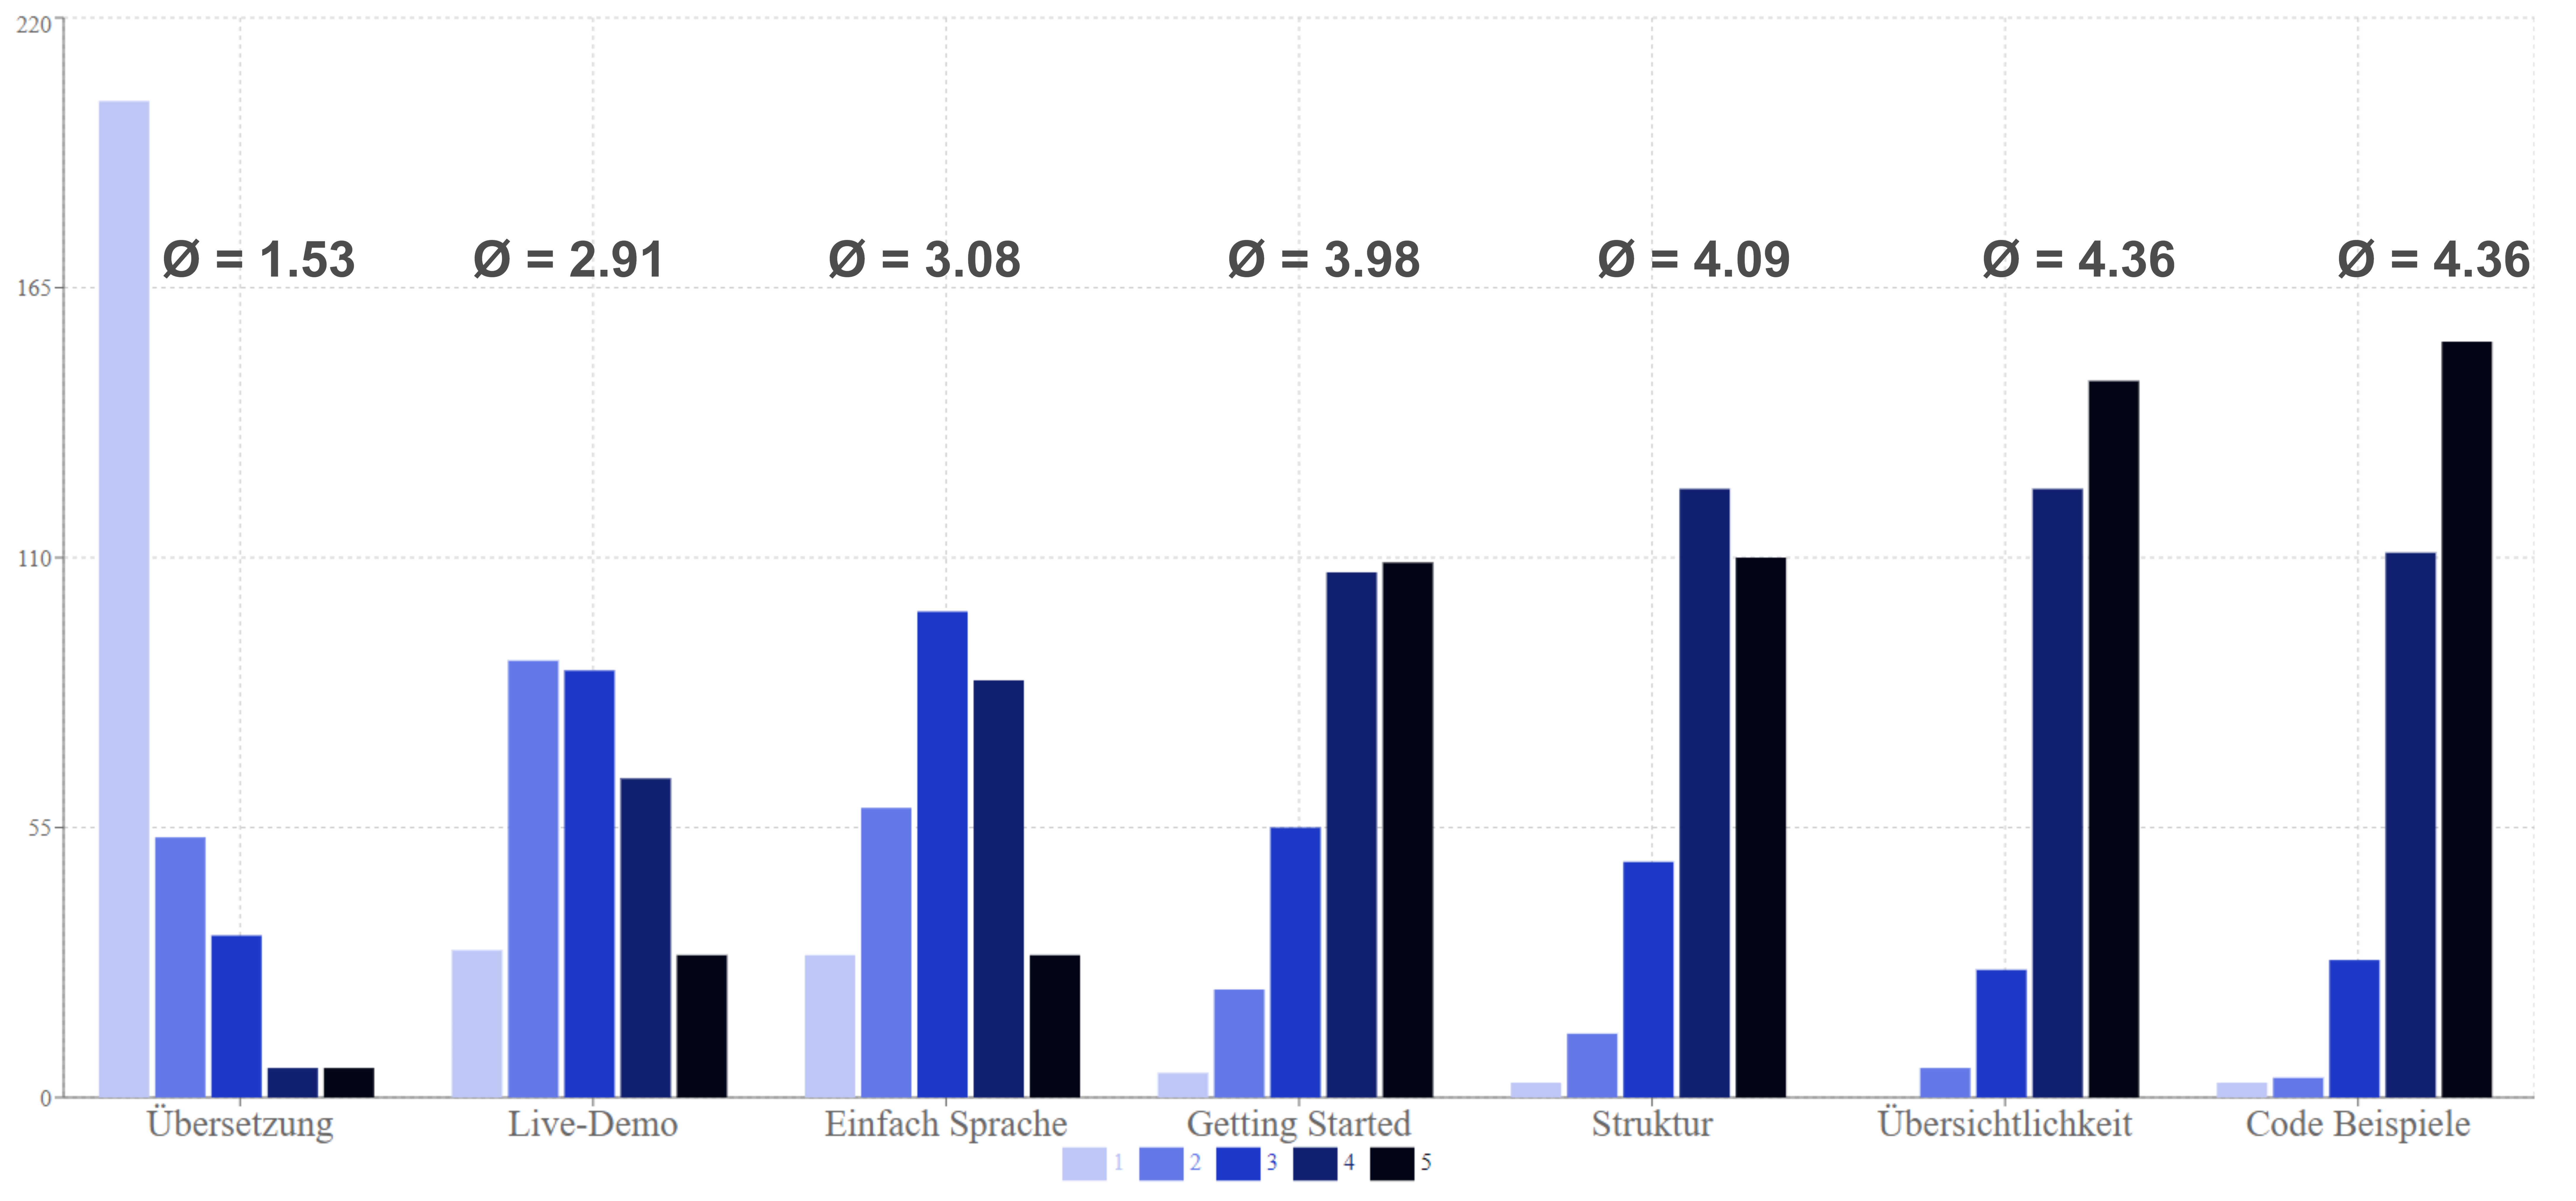
\includegraphics[scale=0.05]{figures/05/GuteDoku_BarChart.png}
    \caption{Antworten: Was zeichnet Gute Dokumentation aus?}
    \label{abb:GuteDoku_BarChart}
\end{figure}

\begin{figure}[h]
    \centering
    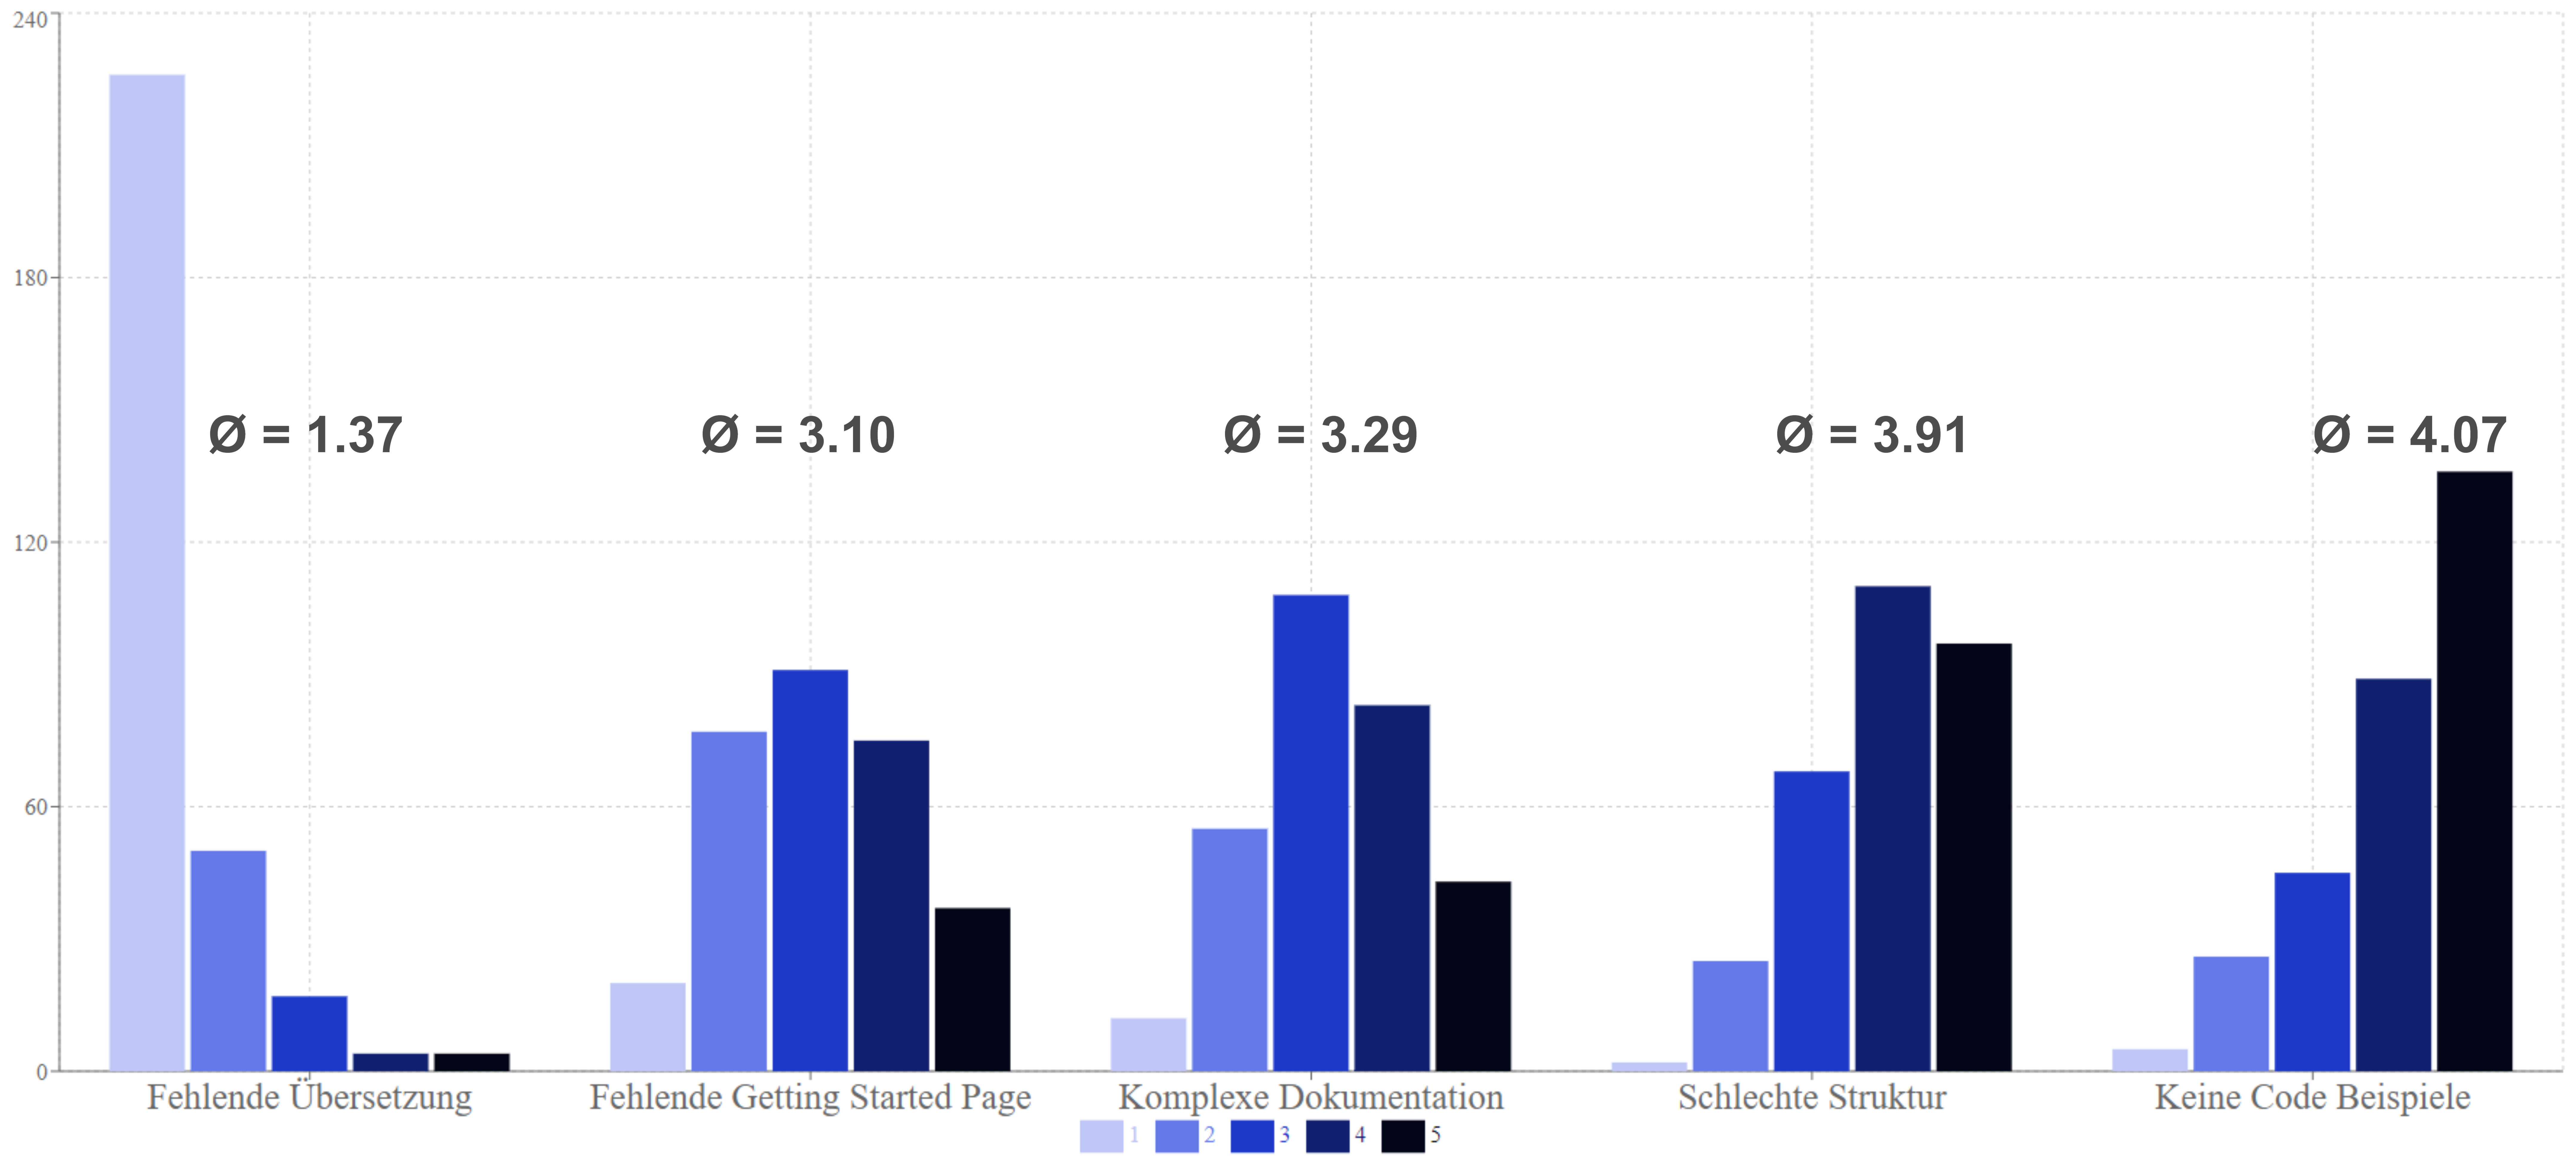
\includegraphics[scale=0.05]{figures/05/SchlechteDoku_BarChart.png}
    \caption{Antworten: Was zeichnet Gute Dokumentation aus?}
    \label{abb:SchlechteDoku_BarChart}
\end{figure}

% Beliebtheit
\newpage
%! newpage
\cleardoublepage %! \cleardoublepage

\section{Beliebtheit}\label{sec:Beliebtheit}
Im zweiten Teil der Umfrage, soll geklärt werden, welchen Einfluss die Beliebtheit, bei der Wahl
eines Projektes hat. Wie zuvor auch sollten die Teilnehmer Kriterien auf einer 5-Punkte Skala bewerten.
Die Mittelwerte der Antworten finden sich in Tabelle \ref{tab:beliebtheit} wieder.

\bigskip
\noindent
Die Aussage war \textit{"Wie sehr achten Sie bei der Auswahl von OSS auf..."}, mit den Punkten:
\begin{multicols}{2}
    \begin{itemize}
        \setlength\itemsep{0em}
        \item Anzahl der GitHub Sterne
        \item Anzahl der Mitwirkenden eines
              Projektes
        \item Anzahl von Sponsoren
        \item Trends
        \item Anzahl an Fragen und Antworten auf\\ StackOverflow
    \end{itemize}
\end{multicols}

\noindent
Diese Punkte wurden gewählt, da es klassischen Vergleichsmerkmalen sind, um die Beliebtheit von OSS
zu vergleichen. GitHub Sterne und Downloads sind eine schnelle und einfache Methode, um die aktuelle 
Beliebtheit eines Projektes zu vergleichen. Trends hingegen stellen GitHub Sterne oder Downloads 
über Zeit dar, häufig genutzte Tools für die Analyse von Trends sind
\textit{StackOverflow Trends}\footnote{\url{https://insights.stackoverflow.com/trends}},
\textit{npm trends}\footnote{\url{https://www.npmtrends.com/}} oder
\textit{Google Trends}\footnote{\url{https://trends.google.de/trends/}}.


% Daten beschreiben
Anders als bei der Dokumentation gibt es hier kein Kriterium mit starker Zustimmung. Die Downloads
sind hierbei mit einer durchschnittlich Zustimmung von 3,27 die beliebtes Vergleichsmetrik für Beliebtheit
gefolgt von Sternen (2,92). Anzahl der Mitwirkenden (2,68), StackOverflow Fragen und Antworten (2,60) sowie 
Trends (2,23) werden tendenziell weniger beachtet. Die Anzahl der Sponsoren wird mit einer durchschnittlichen
Bewertung (1,7) fast gar nicht beachtet. 


Des Weiteren gaben 46\% der Teilnehmer an, dass die geringer Popularität eines Projekts sie schon 
mal davon abgehalten hat dieses zu nutzten.  

% Die leichte Ablehnung der Kriterien deckt sich mit diesem Ergebnissen. Nutzer achten auf Beliebtheit weniger als auf die 
% Qualität der Dokumentation bei der Wahl von OSS.

\begin{table}[h]
    %\resizebox{\textwidth}{!}{%
        \begin{tabular}{cccccc}
            \hline
            Downloads & Sterne & Mitwirkende & StackOverflow Fragen/Antworten & Trends & Sponsoren \\ \hline
            3.27      & 2.92   & 2.68        & 2.60                           & 2.23   & 1.7
        \end{tabular}%
    %}
    \caption{\label{tab:beliebtheit}Einfluss der Beliebtheitsmerkmalen bei der Wahl von OSS}
\end{table}

% Sponsoren %? evtl ganz raus lassen idk...
\newpage
\section{Sponsoren}\label{sec:umfrage_sponsoren}


Im dritten Teil der Umfrage sollte herausgefunden werden, welchen Einfluss Sponsoren bei der OSS Wahl
spielen. Auch hier wurde mit der 5-Punkte Skala bewertet, mit der Frage: \textit{"Bewerten Sie folgende
    Aussagen."} Die Aussagen waren:

\begin{enumerate}
    \setlength\itemsep{0em}
    \item Projekte mit Sponsoren wirken zukunftssicherer
    \item Ich bevorzuge es, wenn möglich, Projekte mit Sponsoren zu nutzten
    \item Gesponserte Projekte sind meistens qualitativ besser
\end{enumerate}

\noindent
Mit einer sehr schwachen Zustimmung von durchschnittlich 3,27 gaben die Teilnehmer an, dass sie 
Projekte mit Sponsoren als zukunftssicherer empfinden. Projekte mit Sponsoren werden tendenziell
weder stark bevorzugt (2,92) noch als qualitativ hochwertiger empfunden (2.68).

\begin{table}[h]
    \begin{tabular}{cccccc}
        \hline
        Aussage: \hspace{1cm} & 1.   & \hspace{0.75cm} & 2.   & \hspace{0.75cm} & 3.   \\ \hline
                              & 3.27 &                 & 2.92 &                 & 2.68
    \end{tabular}%
    \caption{\label{tab:sponsorens}Einfluss von Sponsoren}
\end{table}





% Development
\newpage
\section{Development}
Im vierten Teil der Umfrage ging es um den Einfluss des Entwicklungsprozesses bei der Auswahl von
OSS. Die Frage war: \textit{"Wie sehr achten Sie auf die Folgenden Punkte, wenn Sie ein Projekt
    wählen?"}

\todo{Warum genau diese Punkte?}

\begin{multicols}{2}
    \begin{itemize}
        \setlength\itemsep{0em}
        \item Anzahl aktiver Maintainer
        \item Ticket/Issue Verhältnis Open/Closed
        \item Antwortzeit der Entwickler auf Tickets/Issues
        \item Regelmäßigkeit der Commits
        \item Aktualität des letztes Commit
        \item []
    \end{itemize}
\end{multicols}

\noindent
\todoo{Die gewählten Punkte sind auf GitHub einsehbare Daten, welche als Metriken der Entwicklung
    verwendet werden können.}

\begin{table}[ht]
    %\resizebox{\textwidth}{!}{%
    \begin{tabular}{ccccccc}
        \hline
        Aktualität & Anzahl der Maintainer & Regelmäßigkeit & Verhältnis & Antwortzeit \\ \hline
        3.94       & 3.33                  & 3.28           & 2.90       & 2.86
    \end{tabular}%
    %}
    \caption{\label{tab:development}Einfluss des Entwicklungsprozesses}
\end{table}

\noindent
Ähnlich wie bei der Dokumentation (Sieh Tabellen \ref{tab:freitext_felder_ergebnisse}) legen die Nutzer
einen großen Wert auf Aktualität. \todoo{Gefolgt von Anzahl der Maintainer und Regelmäßigkeit der
    Commits}
Auf Tickets wird hierbei weniger geachtet, weder das Verhältnis zwischen offenen und geschlossen
Tickets noch auf die Antwortzeit der Entwickler auf diese.


\newpage %! new page
\cleardoubleemptypage
\section{Freie Kategorisierung der Erfolgskriterien}\label{sec:umfrage_last_question}


Im letzten Teil der Umfrage sollten die Teilnehmer verschiedene Kriterien per
\textit{Drag and Drop} sortieren. Die Fragestellung lautete
\textit{Sortieren Sie nach den für Sie wichtigsten Kriterien bei der Auswahl von OSS.}
mit folgenden Punkten zum Sortieren


\begin{multicols}{2}
    \begin{itemize}
        \setlength\itemsep{0em}
        \item Gute Dokumentation
        \item Beliebtheit
        \item Anzahl von offenen Issues/Tickets
        \item Trends
        \item Projekt hat Sponsoren
        \item []
    \end{itemize}
\end{multicols}


\noindent
Aufgrund der Übersichtlichkeit hat sich die Auswahl hier auf fünf beschränkt. Es wurde versucht
alle vorherigen Themen abzudecken.
Je nach Platzierung, haben die Kriterien Punkte bekommen, 5 Punkte für den ersten Platz, 4 für den
zweiten usw. der letzte Platz bekam einen Punkt.

Das wichtigste Kriterium ist Gute Dokumentation mit 1329 Punkten, gefolgt von Beliebtheit (1165),
Anzahl der offenen Issues/Tickets (794), Trends (624), Projekt hat Sponsoren (559).

\chapter{Diskussion}

\begin{itemize}
    \item Stichprobe war klein
    \item (Problem => Donations not enough, abhängig was aus dem Crawler für Ergebnisse kommen)
    \item Evtl ist die Stichprobe sehr spezifisch (Überwiegend Studenten)
    \item Fazit => Problem mit Donations? Zu wenige?
          Findet man dieses Problem in den Daten überhaupt... existiert dieses Problem überhaupt
          Soll allerdings nur angeschnitten werden, da die BA nur auf die Sicht der Nutzer geschaut hat.
          Probleme der Open Source Entwickler ist ein anderes Problem.
\end{itemize}
\chapter{Fazit}


%? Was wurde gemacht?
Das Ziel dieser Arbeit war es den Einfluss von \textbf{Lizenzen, Dokumentation, Code of Conduct,
    Contributing Guide, Beliebtheit und Vorhandensein von Sponsoren} zu erforschen. Um dieses Ziel zu
erreichen wurden insgesamt acht Hypothesen aufgestellt. Mithilfe einer Umfrage mit 308 Teilnehmern
sowie einer Datenerhebung von 108 Github Projekten konnten sieben diese Hypothesen belegt werden.

%? Erkenntnisse (1)
Die Umfrage hat gezeigt, dass Dokumentation das wichtigste Entscheidungskriterium der Nutzer bei
der Auswahl von Open Source Software ist. Die wichtigsten Aspekte einer guten Dokumentation sind
hierbei Übersichtlichkeit, Code Beispiele sowie eine Getting Started Seite. Weitere Eigenschaften
sind Aktualität und Vollständigkeit. Die Umfrage kam auf ähnliche Ergebnisse wie \cite{GitHubOpenSourceSurvey2017},
und bestätigt die Aussagen von \cite{scottEightRulesGood2018}
%? Erkenntnisse (2)
Die Umfrage hat auch gezeigt, dass Beliebtheit das zweit wichtigste Entscheidungskriterium ist.
Anzahl der Downloads und die der GitHub Sterne werden hierbei am häufigsten verwendet. Diese Erkenntnis
deckt sich mit der von \cite{midhaFactorsAffectingSuccess2012}.
%? Erkenntnisse (3)
Die Datenerhebung der 108 GitHub Projekte hat gezeigt, dass permissive lizenzierte Projekte einen
höheren Markt- als auch technischen Erfolg zu verzeichnen haben.
Aufgrund der starken Ungleichverteilung der Lizenzen Gruppen, lässt sich allerdings keine allgemeingültigen
Schlussfolgerungen ziehen. 
%? Erkenntnisse (4)
Wie die Datenerhebung und Umfrage gezeigt haben, sind Projekte mit Sponsoren technisch erfolgreicher, als
Projekte ohne. Allerdings haben Sponsoren keinen Einfluss auf den Markterfolg. Sponsoren werden von 
potenziellen Nutzern fast nicht beachtet.

%? Ausblick & Empfehlung für weitere Forschung
Weitere Forschung ist nötig, um den Zusammenhang der von Lizenzen und Erfolg zu erforschen. Hierbei
muss darauf geachtet werden, dass restriktive und permissive Projekte besser gleichverteilt sind.
Da Dokumentation sich als wichtigstes Kriterium des Open Source Erfolgs erwiesen hat, wäre es empfehlenswert
diesen Erfolgsfaktor in weiterer Studien zu untersuchen.
%\end{multicols}

\nocite{*} % Alle verwendeten Quellen angeben.

%? Legacy
%%%%% \chapter{Crawler}

% Beispiel wie Datenanalyse aussehen könnte: 
% https://fossa.com/blog/which-open-source-license-is-the-best-for-commercialization/
% https://docs.github.com/en/code-security/supply-chain-security/understanding-your-software-supply-chain/about-the-dependency-graph#supported-package-ecosystems

% TODO: Formulierungen + Erklären Warum GitHub

% Introduction für den Crawler

Mithilfe des Crawlers kann sowohl der Markterfolg als auch der technische Erfolg gemessen werden.
Über Metriken wie GitHub Sterne, Forks oder Downloads lässt sich der Markterfolg quantifizieren.
Der technische Erfolg findet sich wieder in Daten wie Anzahl an Commits, Frequenz von Commits oder Mitwirkende.

Bei der ersten Recherche wurde festgestellt, dass die Repositories mit den meisten Github Sternen
keine Software direkt sind, sondern Repositories mit Lerninhalten.
Zum Zeitpunkt des Schreibens (13. Februar 2022) werden Platz eins, drei und vier von
\begin{itemize}
    \item freeCodeCamp \textit{(340k Sterne)},
    \item free-programming-books \textit{(222k Sterne)} und
    \item coding-interview-university \textit{(209k Sterne)}
\end{itemize}
belegt.

\bigskip

\noindent
Insgesamt sind unter den Top 10 Repositories auf GitHub nur drei IT Projekte im eigentlichen
Sinne dabei \cite{TopGitHubProjects}.
\begin{itemize}
    \item Vue \textit{(193k Sterne)},
    \item React \textit{(182k Sterne)} und
    \item TensorFlow \textit{(163k Sterne)}.
\end{itemize}


\bigskip
\noindent
Es wird daher nicht möglich sein die Top 100 Projekte für die Datensammlung zu verwenden.
Stattdessen werden Projekte von Hand ausgewählt, um zu garantieren, dass es sich nur um IT Projekte handelt.


% TODO: Jones. 1986 finden und Zitieren, andernfalls muss man schon wieder MID12 Zitieren...
%Zudem wird der Fokus auf JavaScript Projekte liegen. Der Grund hierfür liegt darin, dass
%unterschiedliche Programmiersprachen sich schwerer miteinander vergleichen lassen \todoo{(Jones, 1986)}

% -----------------------------------------------------------------------------------------------------------------


\subsection{Der Crawler}

Hilfreiche Ressourcen:

\begin{itemize}
    \item Welche Daten könnte man erfassen und wie? Sieh \link{https://npms.io/about}{npms.io}.
    \item Hilfreiches Tool: \link{https://www.npmtrends.com/}{npmtrends.com}
    \item API um an NPM Downloads ran zu kommen:
          \link{https://github.com/npm/registry/blob/master/docs/download-counts.md}{GitHub registry}
          bzw.
          \link{https://github.com/npm/download-counts}{Deprecated registry}
\end{itemize}



\subsection{Disclaimer}

npm downloadzahlen sind manipulierbar, ich geh zwar davon aus, dass es allgemein nicht häufig gemacht wird
und da ja sowieso vielmehr in die rechnung rein geht als nur npm downloads. Werden diese daten trotzdem mit erfasst.
\link{https://dev.to/andyrichardsonn/how-i-exploited-npm-downloads-and-why-you-shouldn-t-trust-them-4bme}{How to exploit NPM}.

In einem 
\link{https://blog.npmjs.org/post/92574016600/numeric-precision-matters-how-npm-download-counts-work.html}{Blogpost}
erklärt NPM wie es zu den Download zahlen zustande kommt.


% TODO: Frage
% \frage{
%     Soll ich einzelne Projekte unter die Lupen nehmen, wenn Ja
%     1. Bei der Analyse würde ich auf folgende Punkte eingehen...(*) "reicht das?"
%     2. Wie viele solcher Analysen sollte ich durchführen
% }

% ? Beschränkung auf JS
% \todoo{Ggf. könnte man sich nur auf JavaScript beschränken... Warum?
%     Sieh \cite{midhaFactorsAffectingSuccess2012} Kapitel 4.1 => Verschiedene Sprachen
%     lassen sich schwer miteinander vergleichen.
%     Warum JavaScript? Weil NPM die Anzahl an Downloads anzeigt (Markterfolg) und ich persönlich mich am
%     besten damit auskenne.
%     Java zum Beispiel hat Maven und Gradle. Was das Sammeln von Daten um einiges schwerer machen würde
%     zudem zeigt, Maven keine Downloads zahlen an
%     Market Success vs Technical Success == Download zahlen vs Anzahl an commits in einem Zeitraum.
%     Hierbei lohnt sich ein Blick in \cite{midhaFactorsAffectingSuccess2012} Kapitel 4.2}

% ? What data to collect?
% \begin{itemize}
%     \item Welche Daten werden erhoben
%           \begin{itemize}
%               \item Anzahl an GitHub Stars
%               \item Anzahl an Mitwirkenden
%               \item Anzahl an Commits nach Mitglied => Main Contributor
%               \item Anzahl der Nutzer
%               \item Lizenzen
%               \item Welche Programmiersprache wurde verwendet
%               \item Anzahl an Zeilen commented
%               \item Anzahl an gesamten Commits / Regelmäßigkeit der Commits
%               \item Anzahl der Tickets => Regelmäßigkeit in der Tickets abgearbeitet werden
%               \item Was für ein Projekt ist das? Library/ Framework / Modul / Applikation ... (*)
%               \item Wem gehört das Projekt? Einer Einzelnen Person, einem unabhängigen Team oder einem Unternehmen? (*)
%           \end{itemize}
%     \item evtl. wie wurde der Crawler entwickelt\dots
%     \item Analyse der Daten (Graphen etc.)
%     \item ggf. genauere Analyse von Projekten. Entweder von
%           \begin{itemize}
%               \item den Top Projekte
%               \item Top Projekten aufgeteilt nach Branchen
%           \end{itemize}
%     \item *Diese Punkte müssen ggf. von Hand erhoben werden, das passt dann zum Punkt "Genauere Analyse"
% \end{itemize}

% ? Link zu Top GitHub Projekten
% \href{https://github.com/search?l=&o=desc&q=stars%3A%3E100+stars%3A%3E1&s=stars&type=Repositories}{Link zu Github Top Repos}






 
%%%%% \chapter{Gegenüberstellung der Ergebnisse aus Crawler und Umfrage}

\begin{itemize}
    \item Welche Überschneidungen gibt es
    \item Welche Unterschiede gibt es
    \item Bestätigt das eine das andere?
    \item \dots 
\end{itemize}

\clearpage

% -------------------------------------- Post Chapter Stuff -------------------------------------- %
\appendix

% Print glossaries for used words
%\clearpage
%\printglossaries
%\printnoidxglossaries

\cleardoublepage


\bibliographystyle{natger}
% \bibliographystyle{ieeetr} % Alternative gäbe es halt noch IEEE, würde aber von der Vorlage abweichen
\bibliography{thesis}

\cleardoublepage
\footnotesize
\printindex


\end{document}
